\documentclass[12pt,t]{beamer}
\usepackage{hyperref}
\usepackage{localbeamer}
\usepackage{amsmath,amssymb}

\graphicspath{{./figures/}}

%\newtheorem{definition}{Definition}
%\newtheorem{example}{Example}
%\newtheorem{theorem}{Theorem}
%\newtheorem{lemma}{Lemma}
\DeclareMathOperator{\erf}{erf} \DeclareMathOperator{\prob}{Prob}


\begin{document}

\title[Optimal Microfluidic Mixing and Cutoff]{Cutoffs in Chaotic Map Mixing and \\Topology Optimization of Microfluidic Channels}
\author{Tzu-Chen Liang}
\institute[Stanford University]%
{Aeronautics and Astronautics, Stanford University\\
\url{http://www.stanford.edu/~tzuchen/}} \coauthor{Advised by Matthew West}
\date{December 6, 2007}
\frame{\titlepage}

%%%%%%%%%%%%%%%%%%%%%%%%%%%%%%%%%%%%%%%%%%%%%%%%%%%%%%%%%%%%%%%%%%%%%%%
\begin{frame}
  \myframetitle{Microfluidic Mixing}
  \begin{itemize}
  \item Water in channel with cross-section $\ell \approx 100\,\mu\text{m}$.
  \item Reynolds number $\text{Re} = U\ell/\nu < 100$.
  \item P\'eclet number $\text{Pe} = U\ell/D \approx 10^6$.
  \item Required mixing channel length $\approx 1000\,\text{cm}$.
  \end{itemize}
  \begin{center}
      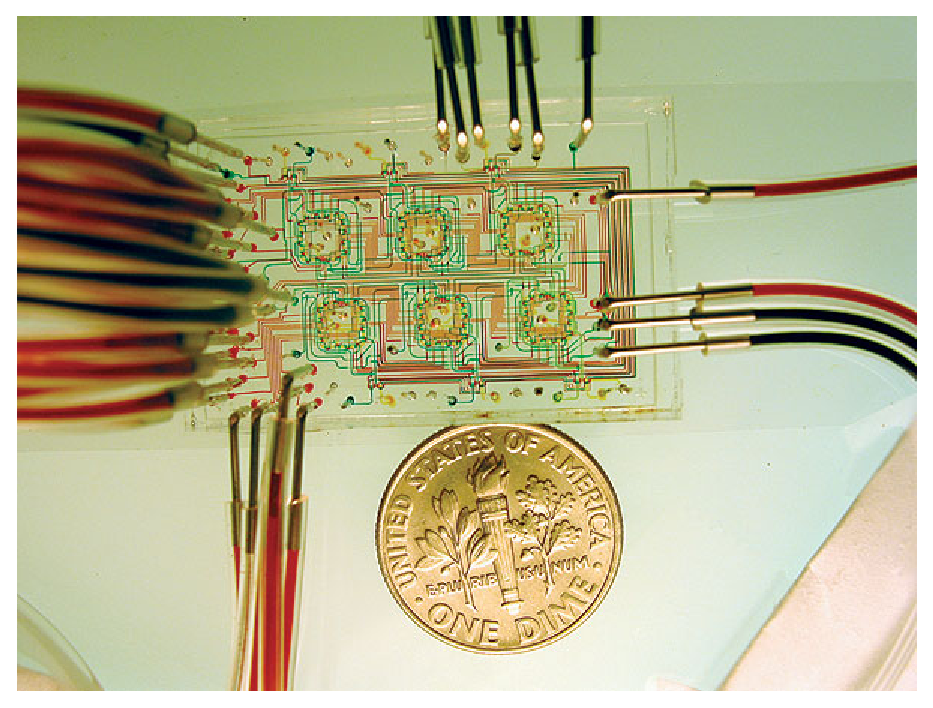
\includegraphics[width=0.50\textwidth]{microfluidicmixer}\\[-0cm]
      \tiny{Whitesides, \textit{Nature} \textbf{442} (2006)}
  \end{center}
  
\end{frame}



%%%%%%%%%%%%%%%%%%%%%%%%%%%%%%%%%%%%%%%%%%%%%%%%%%%%%%%%%%%%%%%%%%%%%%%%%
\begin{frame}
\myframetitle{Stroock's Staggered Herringbone Mixer}
%%%%%%%%%%%%%%%%%%%%%%%%%%%%%%%%%%%%%%%%%%%%%%%%%%%%%%%%%%%%%%%%%%%%%%%%%
%%%%%%%%%%%%%%%%%%%%%%%%%%%%%%%%%%%%%%%%%%%%%%%%%%%%%%%%%%%%%%%%%%%%%%%%%
  \begin{figure}
    \centerline{
     \includegraphics[width=0.58\textwidth]{stroockmixer2}
     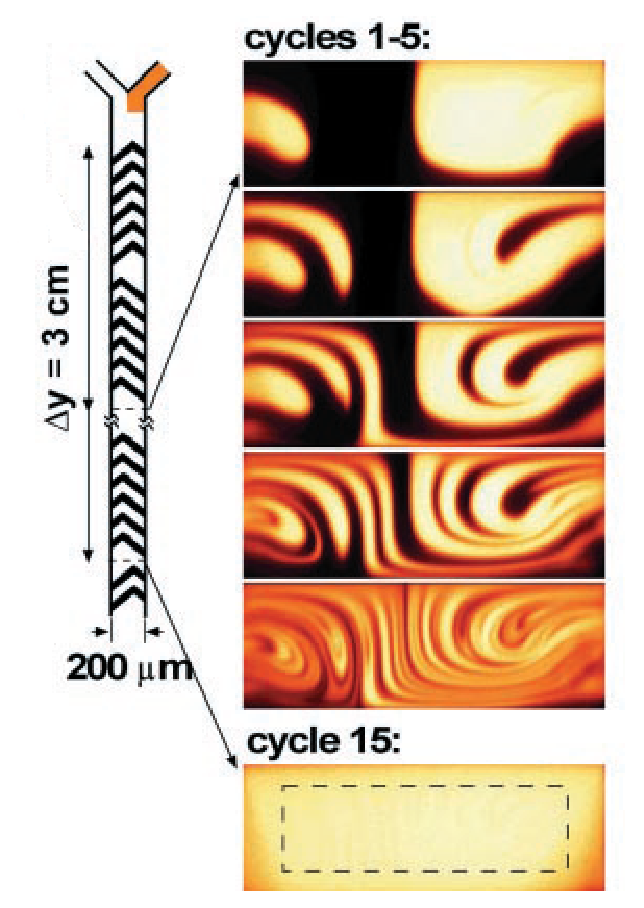
\includegraphics[width=0.21\textwidth]{stroockcrosssection}
     %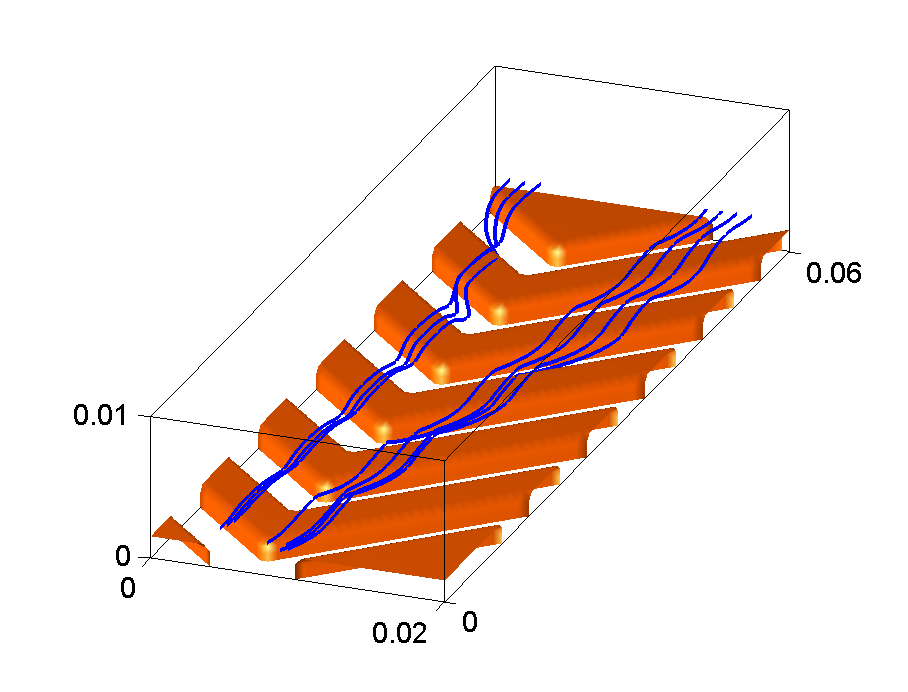
\includegraphics[width=0.35\textwidth]{stroockstructure}
    }
  \end{figure}
  \vspace{-0.3cm}
  \begin{itemize}
    \item Stroock, Dertinger, Ajdari, Mezi\'c, Stone, Whitesides, \textit{Science} \textbf{295} (2002).
    \item Mixing length grows linearly with $\log(\text{Pe})$.
    \item Our goal: improve it by applying topology optimization on the half-cycle structure.
  \end{itemize}
\end{frame}

%%%%%%%%%%%%%%%%%%%%%%%%%%%%%%%%%%%%%%%%%%%%%%%%%%%%%%%%%%%%%%%%%%%%%%%
%%%%%%%%%%%%%%%%%%%%%%%%%%%%%%%%%%%%%%%%%%%%%%%%%%%%%%%%%%%%%%%%%%%%%%%
\begin{frame}
\myframetitle{Model the Structured Channel}
 \begin{itemize}
  \item Topology optimization rather than shape optimization. 
  \item Generalized Stokes partial differential equation for imcompressible flow (Darcey equation),
       \begin{eqnarray*}
          \begin{aligned}
        ( -\nu\Delta + \alpha ) u +\nabla  p & = f\\
        \text{div} u& =  0
          \end{aligned}
       \end{eqnarray*}

       $u(x)$: velocity, $p(x)$: pressure, $f$: body force and boundary conditions, $\nu$: kinematic viscosity, and $\alpha(x)$: inverse permeability
 \item Allow porous material: a relaxation.
 \item Assumptions: velocity field is fully developed, periodic boundary condition.
  \end{itemize}
\end{frame}
%%%%%%%%%%%%%%%%%%%%%%%%%%%%%%%%%%%%%%%%%%%%%%%%%%%%%%%%%%%%%%%%%%%%%%%
%%%%%%%%%%%%%%%%%%%%%%%%%%%%%%%%%%%%%%%%%%%%%%%%%%%%%%%%%%%%%%%%%%%%%%%
\begin{frame}
  \myframetitle{Objective Functions}
  \begin{itemize}
    \item Can't really minimize our performance measure ``mixing length''.
    \vspace{-0.3cm}
    \begin{itemize}
          \item Mixing length ($x_{90}$): the channel length required for the standard deviation of the color on the cross-section of the channel dropping by 90\%.
    \end{itemize}
    \item Alternatives:
       \begin{itemize}
          \item A linear function of velocity $g(u) = c^Tu$: maximize the downward velocity between the two vortices.
          \item A distance measure between the current flow map and a desired flow map.
          \item The ``mixing rate'' of a Markov Chain: the spectral gap $1-|\lambda_2|$.
       \end{itemize}
  \end{itemize}
\end{frame}
%%%%%%%%%%%%%%%%%%%%%%%%%%%%%%%%%%%%%%%%%%%%%%%%%%%%%%%%%%%%%%%%%%%%%%%
%%%%%%%%%%%%%%%%%%%%%%%%%%%%%%%%%%%%%%%%%%%%%%%%%%%%%%%%%%%%%%%%%%%%%%%
\begin{frame}
  \myframetitle{Simulation: A Markov Chain Model}
  \begin{itemize}
     \item Advection-Diffusion Equation.
        \begin{eqnarray*}
           \label{ade}
            u \cdot \nabla \phi = D \Delta \phi
        \end{eqnarray*}
     where $\phi(x)$: the color intensity, and $u(x)$: the velocity field. 
     \item A Markov Chain model to approximate $f^k = \phi|_{\text{cross-section } k}$.
       \begin{tabular}{cl}
         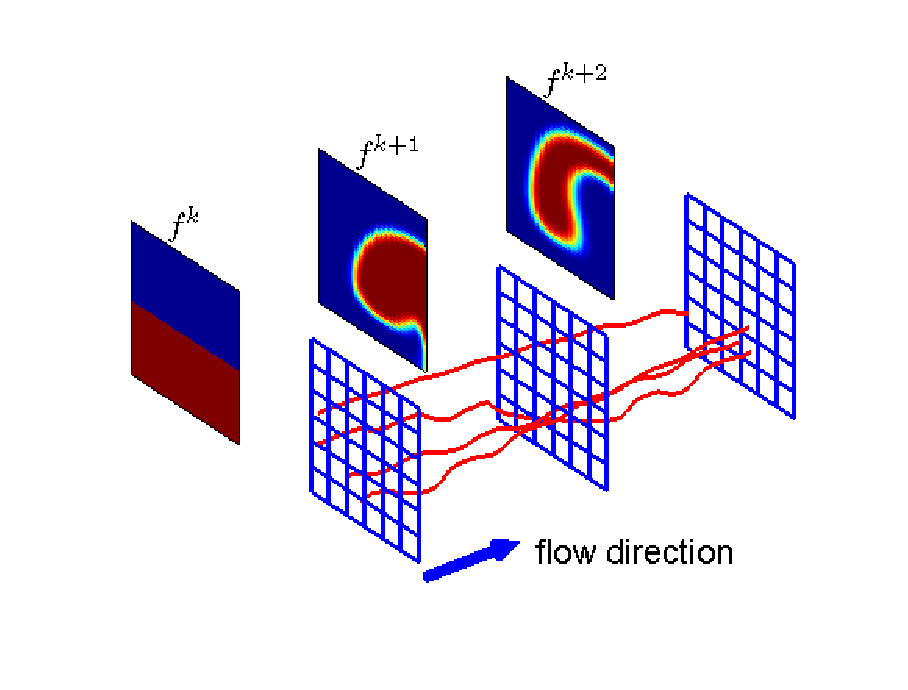
\includegraphics[width=0.4\textwidth,trim=2cm 0cm 1cm 0cm,clip]{markovchainmodel}
      %  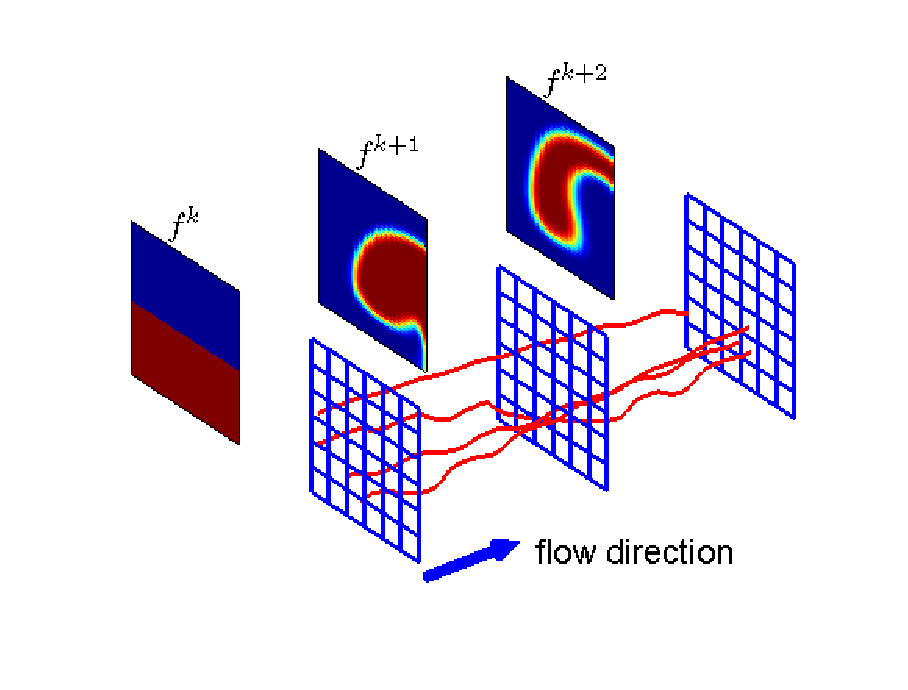
\includegraphics[width=0.4\textwidth,trim=2cm 0cm 1cm 0cm,clip]{markovchainmodel}&
        \begin{minipage}[b]{6.2cm}
           \begin{itemize}
             \item $P_{ij} = \prob(x^{k}=j \mid x^{k+1}=i)$
             \item Perron-Frobenius Operator: $\omega^{k} = P^T \omega^{k+1}$ 
             \item Koopman Operator: $f^{k+1} = P f^{k}$
             \item Use $800 \times 1600$ grids. $D\approx 10^{-11}\,\text{cm}^2$ per iteration.  
           \end{itemize}
        \end{minipage}
       \end{tabular}
  \end{itemize}


\end{frame}

%%%%%%%%%%%%%%%%%%%%%%%%%%%%%%%%%%%%%%%%%%%%%%%%%%%%%%%%%%%%%%%%%%%%%%%
%%%%%%%%%%%%%%%%%%%%%%%%%%%%%%%%%%%%%%%%%%%%%%%%%%%%%%%%%%%%%%%%%%%%%%%
\begin{frame}
\myframetitle{Without and With Diffusion}
\begin{center}
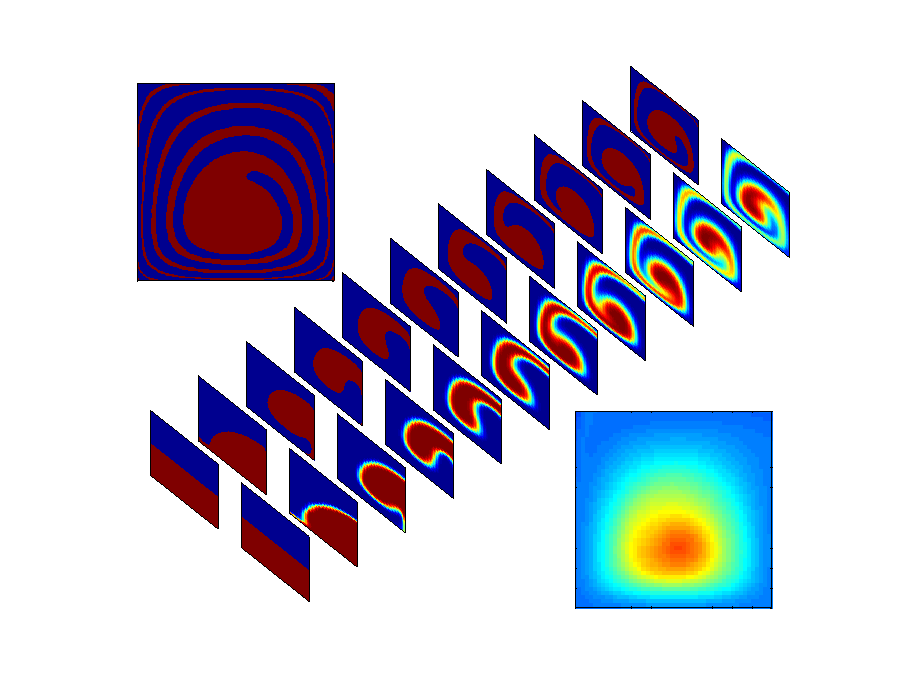
\includegraphics[width=0.83\textwidth,trim=0cm 1cm 0cm 0.5cm,clip]{markovvsexact}
\end{center}
\end{frame}

%%%%%%%%%%%%%%%%%%%%%%%%%%%%%%%%%%%%%%%%%%%%%%%%%%%%%%%%%%%%%%%%%%%%%%%
%%%%%%%%%%%%%%%%%%%%%%%%%%%%%%%%%%%%%%%%%%%%%%%%%%%%%%%%%%%%%%%%%%%%%%%
\begin{frame}
\myframetitle{Without and With Diffusion}
\centerline{
%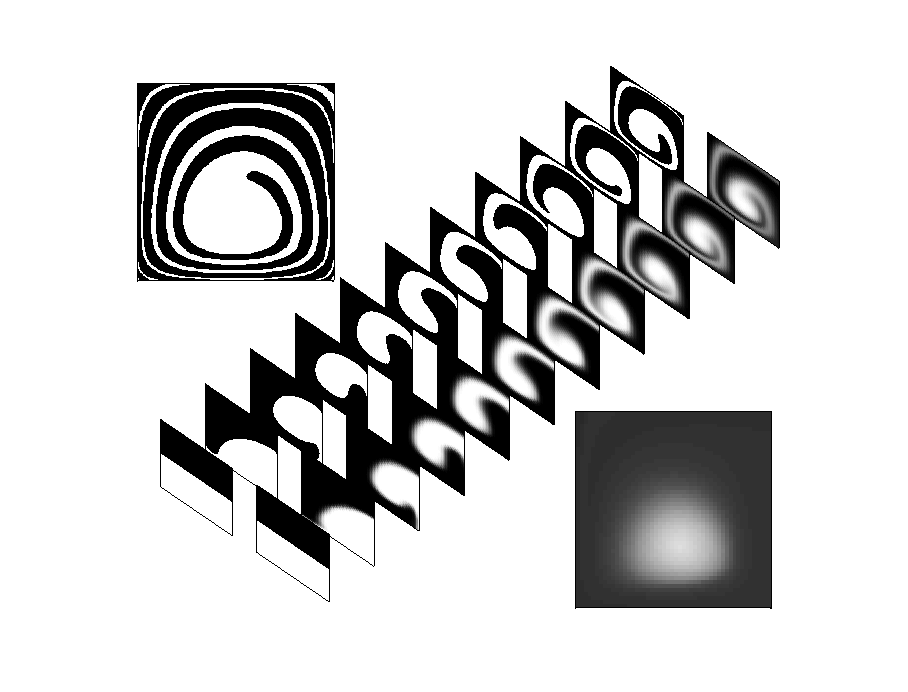
\includegraphics[width=0.8\textwidth,trim=1cm 1cm 0cm 0.5cm,clip]{markovvsexact2}
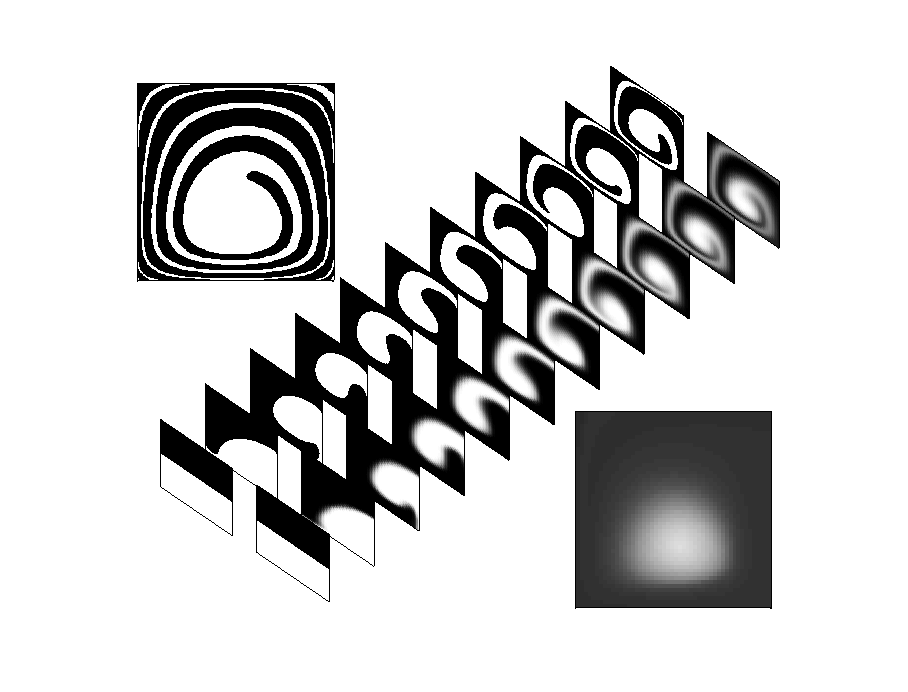
\includegraphics[width=0.8\textwidth,trim=1cm 1cm 0cm 0.5cm,clip]{markovvsexact2}
}

\end{frame}

%%%%%%%%%%%%%%%%%%%%%%%%%%%%%%%%%%%%%%%%%%%%%%%%%%%%%%%%%%%%%%%%%%%%%%%
%%%%%%%%%%%%%%%%%%%%%%%%%%%%%%%%%%%%%%%%%%%%%%%%%%%%%%%%%%%%%%%%%%%%%%%
\begin{frame}
\myframetitle{Topology Optimization and Adjoint Method} The optimization
\begin{align*}
      \text{minimize } & g(u,p,\alpha) \\
      \text{subject to } & \begin{bmatrix} -\nu L + \alpha H & G \\
        D & 0 \end{bmatrix} \begin{bmatrix} u \\ p \end{bmatrix}
      = \begin{bmatrix} f \\ 0 \end{bmatrix} \\
      & 0 \le \alpha \le \alpha_{\text{max}}\\
\end{align*}
Compute gradient with adjoint of constraint $R(u,p,\alpha) = 0$
\begin{align*}
      \frac{d g}{d \alpha} &= \frac{\partial g}{\partial \alpha}
      + \frac{\partial g}{\partial u} \frac{\partial u}{\partial \alpha}   
         \begin{picture}(10,5)\put(16,9){\vector(-2,-1){13}} \put(16,9){\footnotesize{dense}} \end{picture}
      &
      \frac{d R}{d \alpha} = \frac{\partial R}{\partial \alpha}
      + \frac{\partial R}{\partial u} \frac{\partial u}{\partial \alpha}
      &= 0 \\
      &= \frac{\partial g}{\partial \alpha}
      - \underbrace{\frac{\partial g}{\partial u}
      \left(\frac{\partial R}{\partial u}\right)^{-1}}_{x^T}
      \frac{\partial R}{\partial \alpha} 
      \begin{picture}(10,5)\put(16,9){\vector(-2,-1){13}} \put(17,9){\footnotesize{sparse}}  \put(45,9){\vector(3,-1){24}}\end{picture}
      &
      \left( \frac{\partial R}{\partial u} \right)^T x
      &= \left(\frac{\partial g}{\partial u} \right)^T
\end{align*}

\end{frame}




%%%%%%%%%%%%%%%%%%%%%%%%%%%%%%%%%%%%%%%%%%%%%%%%%%%%%%%%%%%%%%%%%%%%%%%
%%%%%%%%%%%%%%%%%%%%%%%%%%%%%%%%%%%%%%%%%%%%%%%%%%%%%%%%%%%%%%%%%%%%%%%
\begin{frame}
  \myframetitle{Methods and Tools}
  Methods
  \begin{itemize}
   \item Finite difference method with staggered mesh to solve the flow field ($180 \times 30 \times 60$ fluid/structure grid).
   \item Adjoint method to find $\frac{dg}{d\alpha}$ without forming $\frac{du}{d\alpha}$.
   \item A gradient-based optimization scheme with fixed step size.
   \item A Markov Chain model to approximate the solution of the advection-diffusion equation on the cross-sections of the channel.
   \item Fourth order Runge-Kutta method to integrate streamlines.
   \end{itemize}
   Tools
   \begin{itemize}
   \item PETSc (Portable, Extensible Toolkit for Scientific Computation).
   %\item Develope a package that communicates PETSc and Matlab
   \item 72-node cluster, 1GB RAM/CPU, gigabit ethernet.
   \end{itemize}
\end{frame}



%%%%%%%%%%%%%%%%%%%%%%%%%%%%%%%%%%%%%%%%%%%%%%%%%%%%%%%%%%%%%%%%%%%%%%%
%%%%%%%%%%%%%%%%%%%%%%%%%%%%%%%%%%%%%%%%%%%%%%%%%%%%%%%%%%%%%%%%%%%%%%%
\begin{frame}
\myframetitle{Optimal $2$-D and $3$-D Structures}
  \begin{figure}
    \centerline{
    \begin{tabular}{cc}
      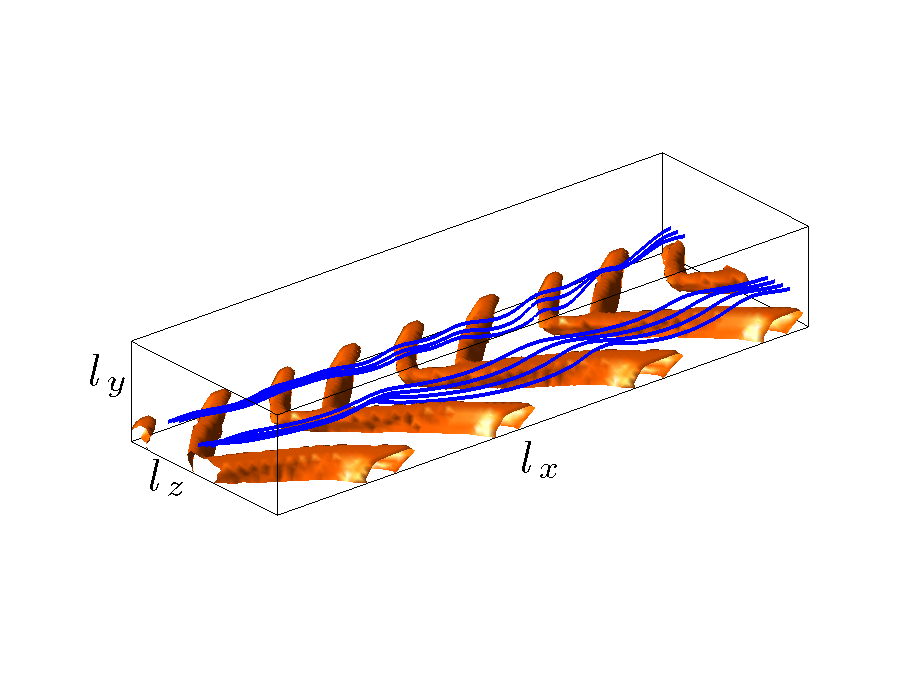
\includegraphics[width=0.4\textwidth,trim=1cm 0cm 1cm 1.6cm,clip]{example2structureherringbone}&
       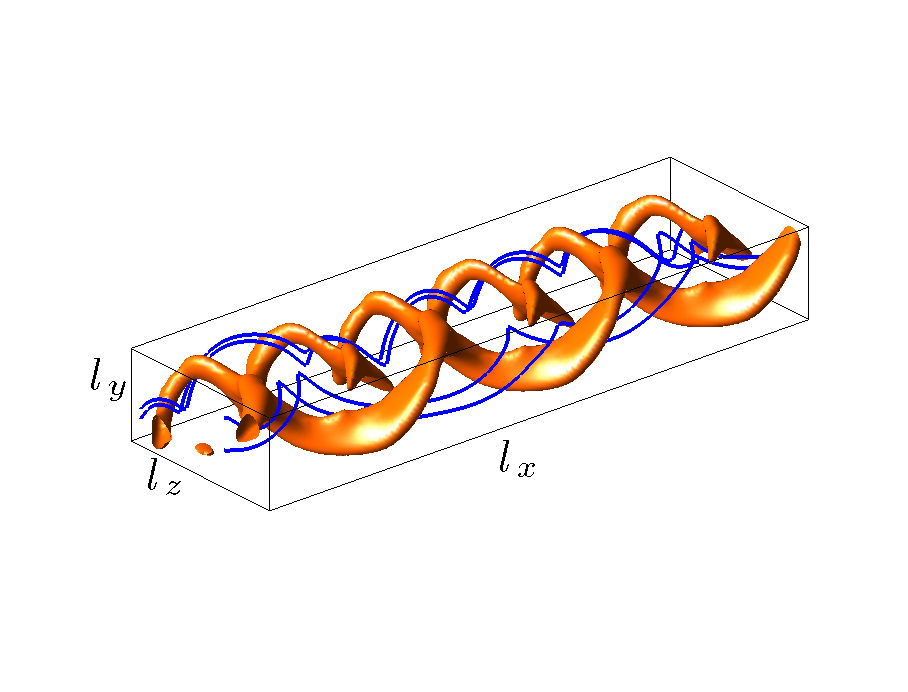
\includegraphics[width=0.4\textwidth,trim=1cm 0cm 1cm 1.6cm,clip]{example2structure3d}\\[-0.7cm]
      \footnotesize{Optimal herringbone channel} & \footnotesize{Optimal 3-D structured channel}
    \end{tabular} 
    }
  \end{figure}
%\vspace{-1cm}
  \begin{itemize}
  \item $(l_x,l_y,l_z)=(0.06,0.01,0.02)\,\text{cm}$.
  \item Solutions are feasible for the non-relaxed problem. 
  \item Non-trivial $3$-D geometry.
     \begin{itemize}
      \item Harder to fabricate with photolithography?
      \item Requires higher pressure for the same flow velocity.
     \end{itemize}
\end{itemize}
\end{frame}

%%%%%%%%%%%%%%%%%%%%%%%%%%%%%%%%%%%%%%%%%%%%%%%%%%%%%%%%%%%%%%%%%%%%%%%
%%%%%%%%%%%%%%%%%%%%%%%%%%%%%%%%%%%%%%%%%%%%%%%%%%%%%%%%%%%%%%%%%%%%%%%
\begin{frame}
\myframetitle{Build a Full Cycle}
  \begin{itemize}
    \item A full cycle of mixing channel is composed of two half-cycle channels.
    \item We try different number of periodic structures per half-cycle to find the best combination.
  \end{itemize}
  \begin{figure}
       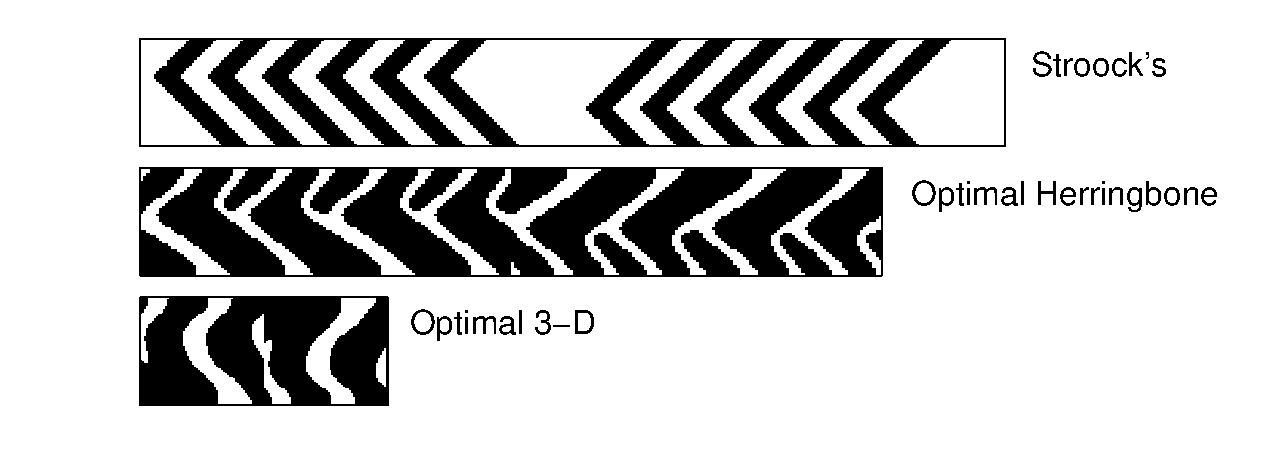
\includegraphics[width=0.9\textwidth,trim=0cm 0cm 0cm 0cm,clip]{example2fullcycle}
  \end{figure}
\end{frame}


%%%%%%%%%%%%%%%%%%%%%%%%%%%%%%%%%%%%%%%%%%%%%%%%%%%%%%%%%%%%%%%%%%%%%%%%%
%%%%%%%%%%%%%%%%%%%%%%%%%%%%%%%%%%%%%%%%%%%%%%%%%%%%%%%%%%%%%%%%%%%%%%%%%
\begin{frame}
 \myframetitle{How Chaotic Mixing Works}
    \begin{center}
      \includegraphics[width=0.65\textwidth]{chaoticmixing}
    \end{center}
Three-stage transition on the variance trajectory.

\end{frame}
%%%%%%%%%%%%%%%%%%%%%%%%%%%%%%%%%%%%%%%%%%%%%%%%%%%%%%%%%%%%%%%%%%%%%%%
%%%%%%%%%%%%%%%%%%%%%%%%%%%%%%%%%%%%%%%%%%%%%%%%%%%%%%%%%%%%%%%%%%%%%%%
\begin{frame}
\myframetitle{Mixing Length}
    \begin{center}
       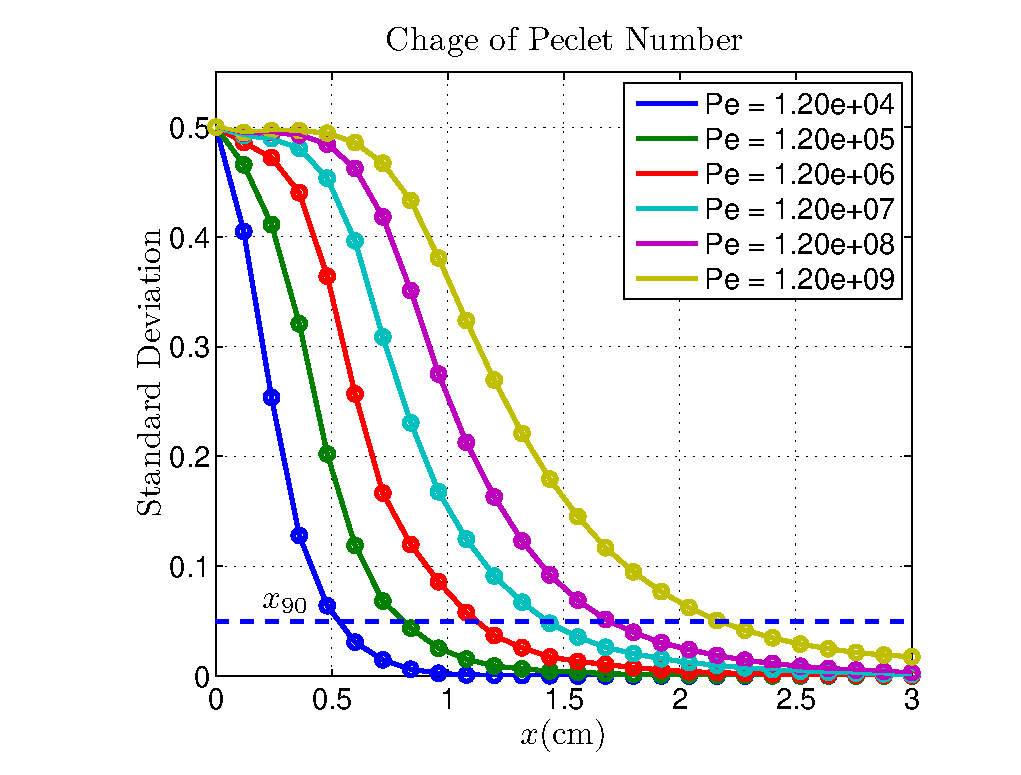
\includegraphics[width=0.47\textwidth]{example2veryPe2}
       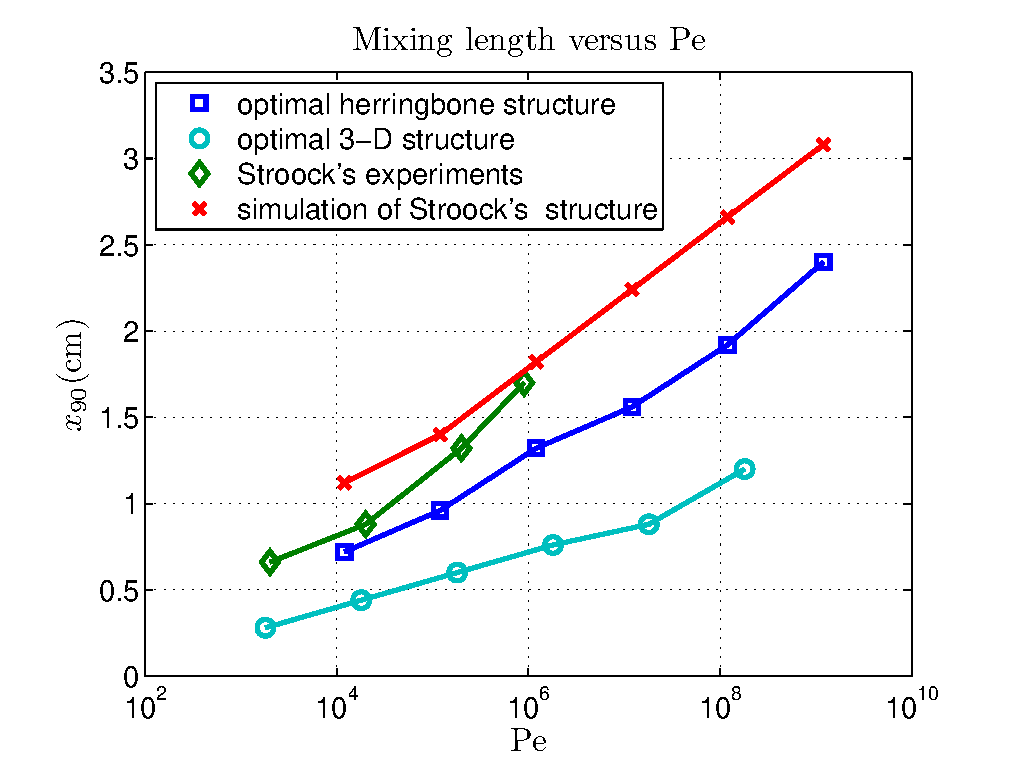
\includegraphics[width=0.47\textwidth]{example2mixinglength2}
    \end{center}
  \begin{itemize}
    \item Mixing Length ($x_{90}$) grows linearly with $\log(\text{Pe})$.
    \item Improvement: 
        \begin{itemize}
        \item 30\% by optimal herringbone structure. 
        \item 60\% by optimal $3$-D structure.
        \end{itemize}
  \end{itemize}
\end{frame}


%%%%%%%%%%%%%%%%%%%%%%%%%%%%%%%%%%%%%%%%%%%%%%%%%%%%%%%%%%%%%%%%%%%%%%%
%%%%%%%%%%%%%%%%%%%%%%%%%%%%%%%%%%%%%%%%%%%%%%%%%%%%%%%%%%%%%%%%%%%%%%%
%\begin{frame}
%\myframetitle{Why not Minimize $|\lambda_2|$?}
%  \begin{itemize}
%    \item Left: Strook's experiment; right: Our simulation.
%    \begin{center}
%     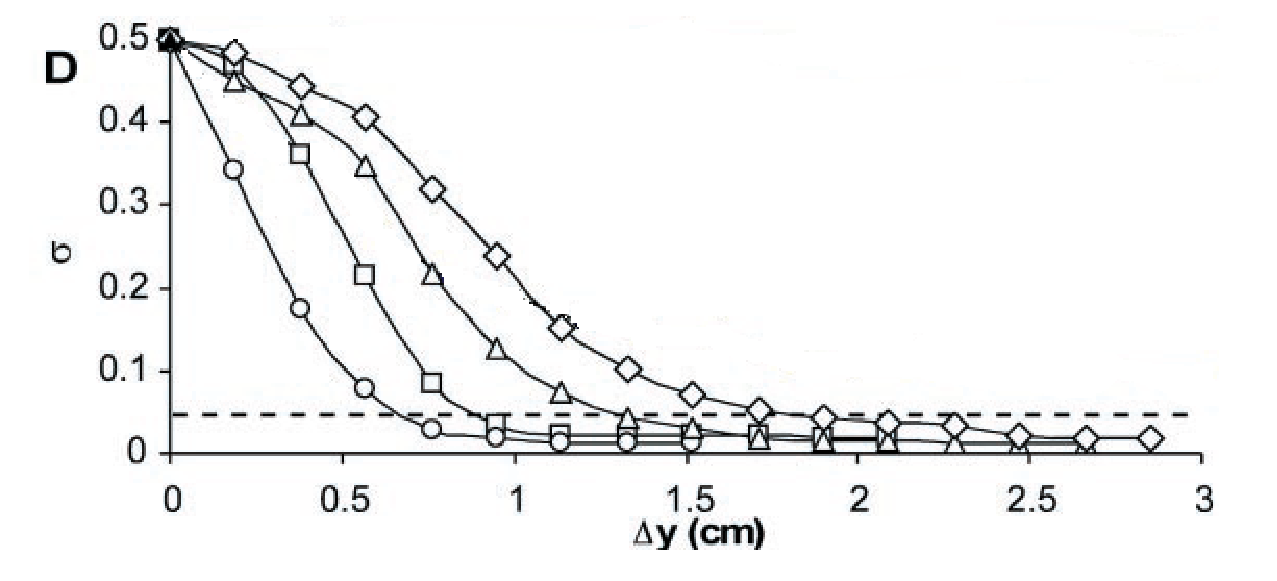
\includegraphics[width=0.3\textwidth,height=0.22\textwidth]{stroockexperiment}
%     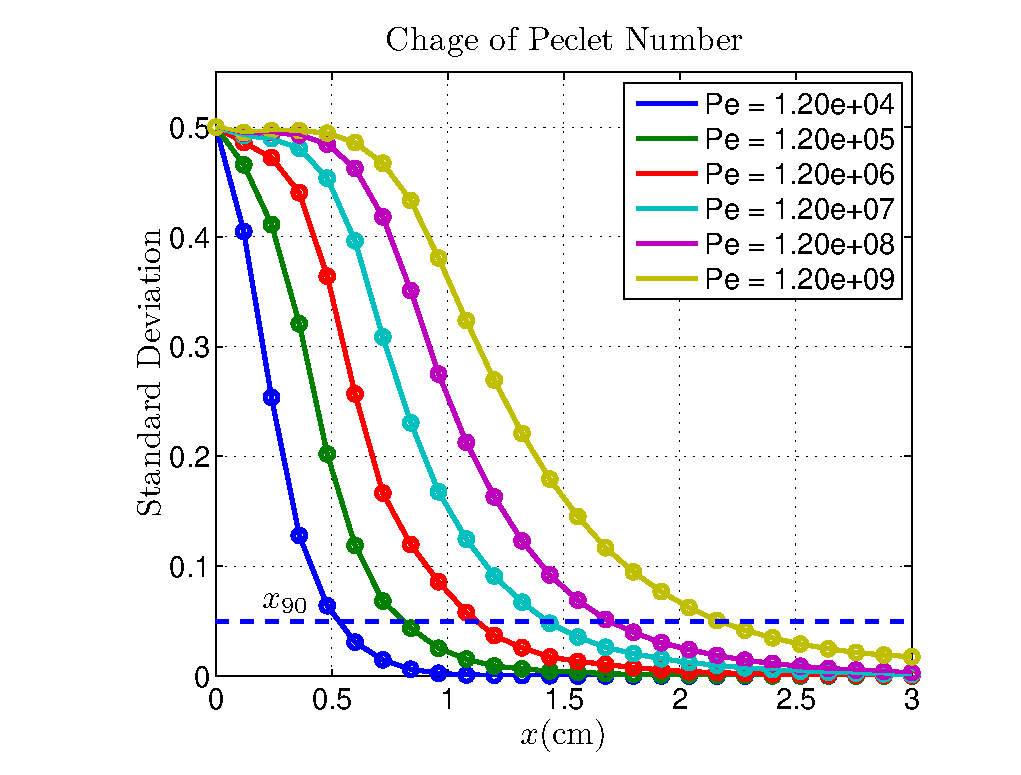
\includegraphics[width=0.3\textwidth]{example2veryPe2}
%    \end{center}
%    \item Left: J-L Thiffeault, 2006, Modified Cap Map simulation;    Right: J. P. Gleeson, 2005, Standard map simulation(log scale).
%   \begin{center}
%       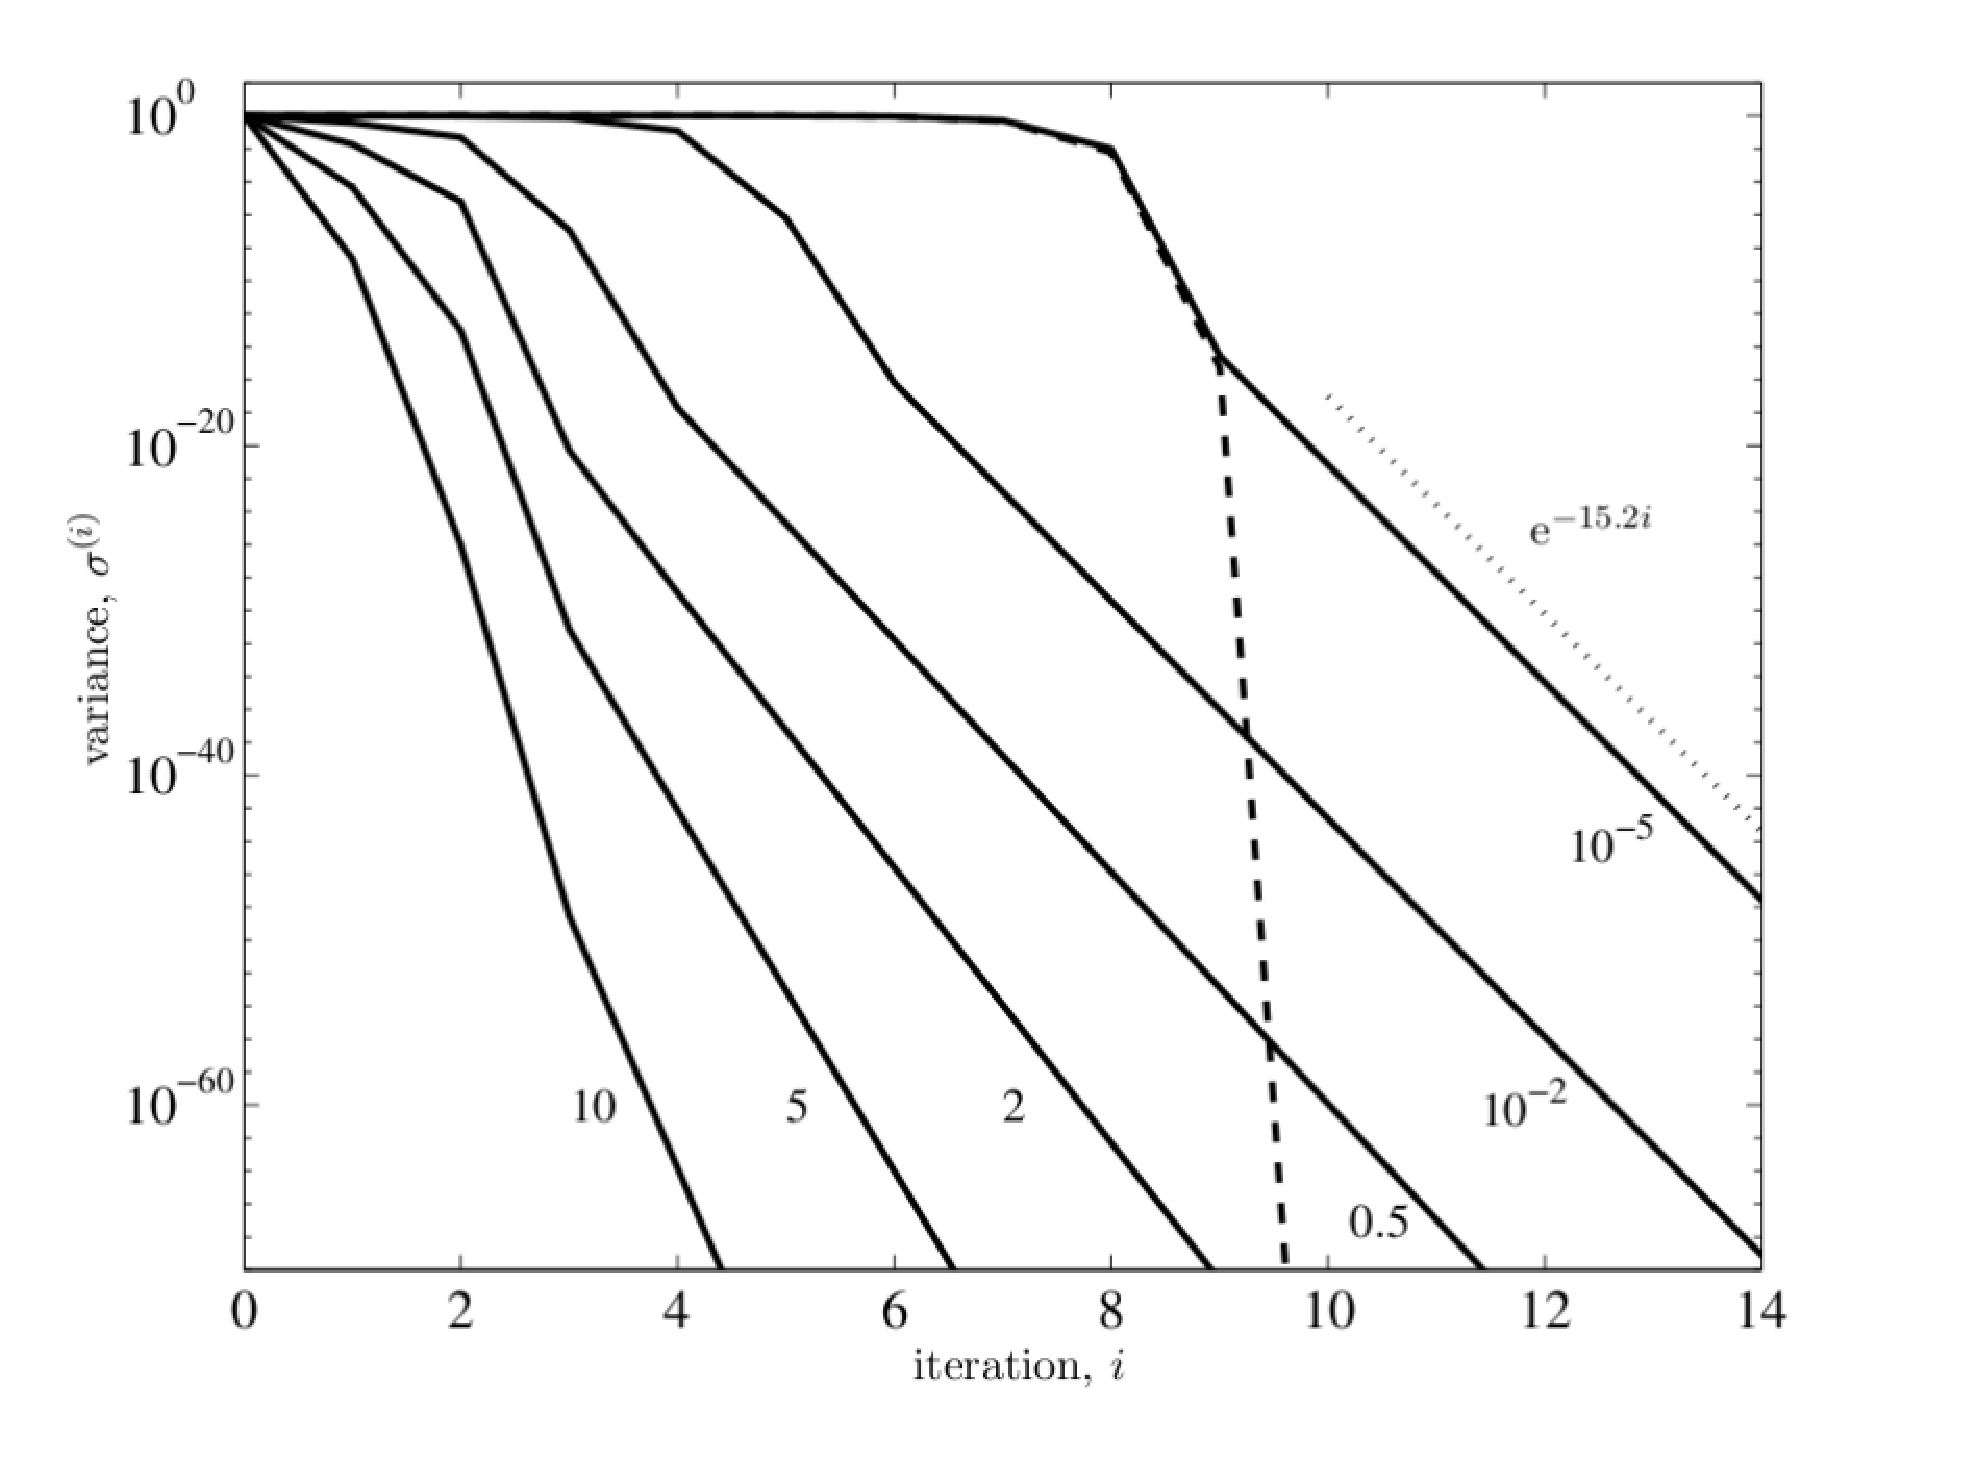
\includegraphics[width=0.3\textwidth]{catmap}
%       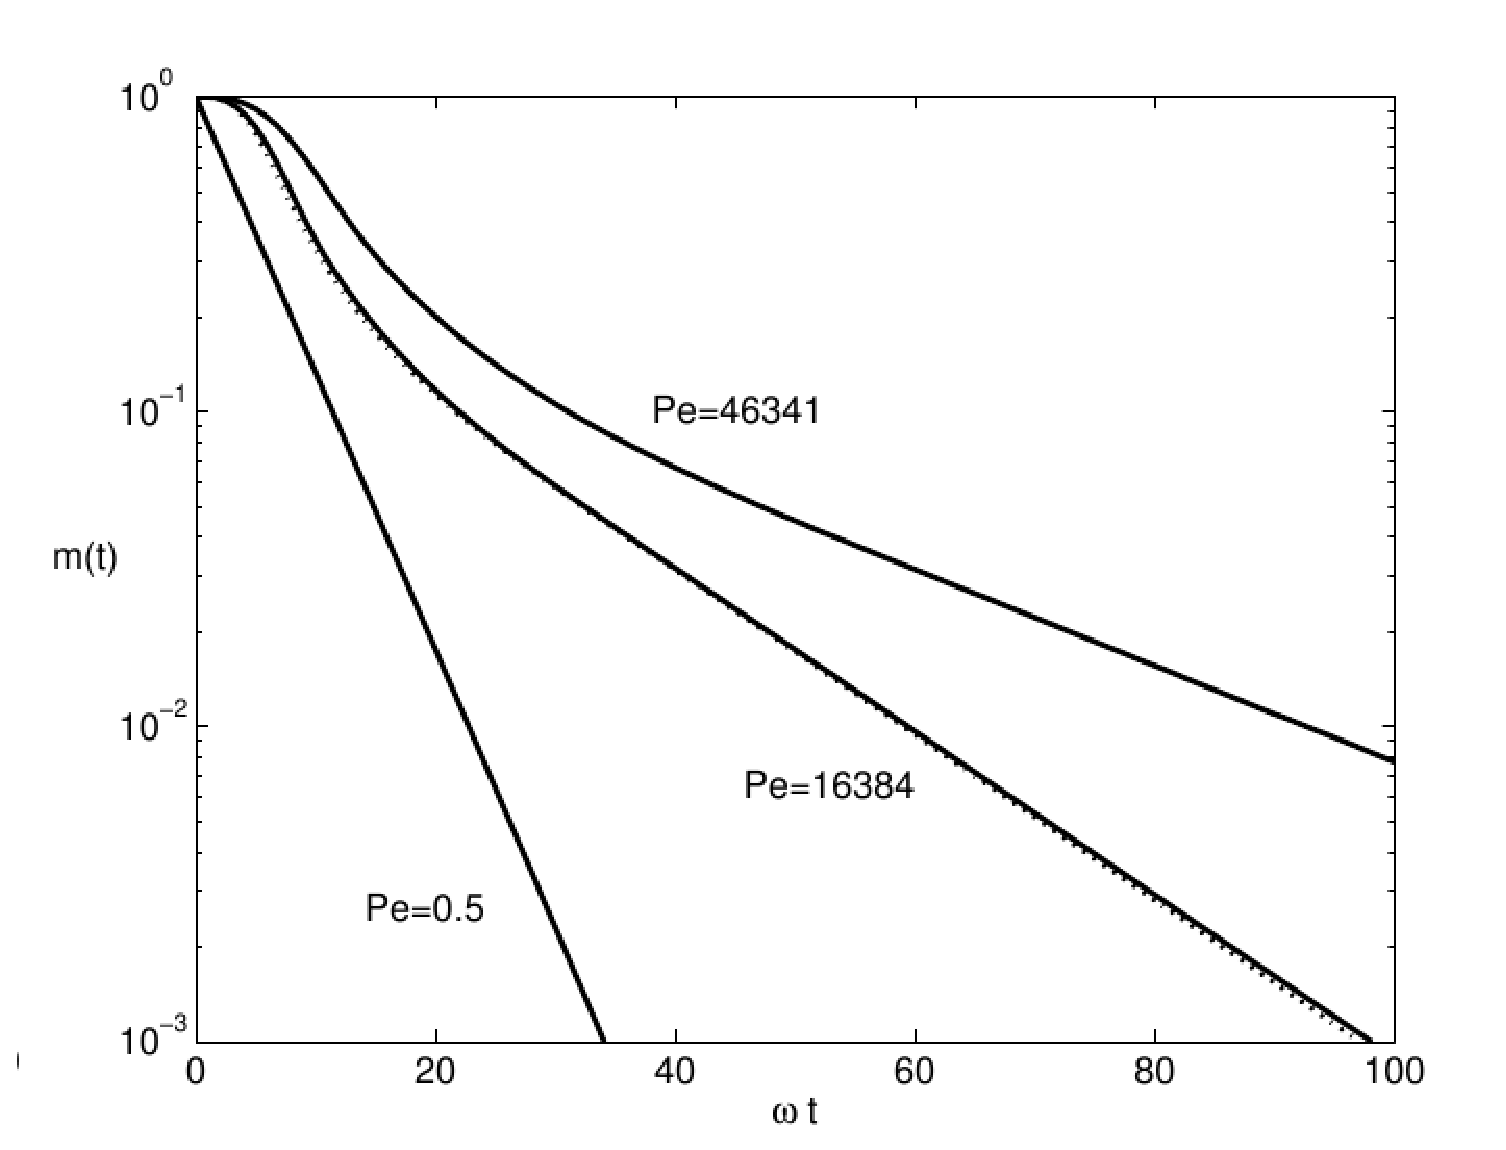
\includegraphics[width=0.3\textwidth]{Glessonstandardmap}
%    \end{center}
%\end{itemize}
%\end{frame}

%%%%%%%%%%%%%%%%%%%%%%%%%%%%%%%%%%%%%%%%%%%%%%%%%%%%%%%%%%%%%%%%%%%%%%%
%%%%%%%%%%%%%%%%%%%%%%%%%%%%%%%%%%%%%%%%%%%%%%%%%%%%%%%%%%%%%%%%%%%%%%%
\begin{frame}
\myframetitle{Why Not Minimize $|\lambda_2|$?}
  \begin{itemize}
    \item The mixing trajectories in log scale.
  \end{itemize}
    \begin{center}   
     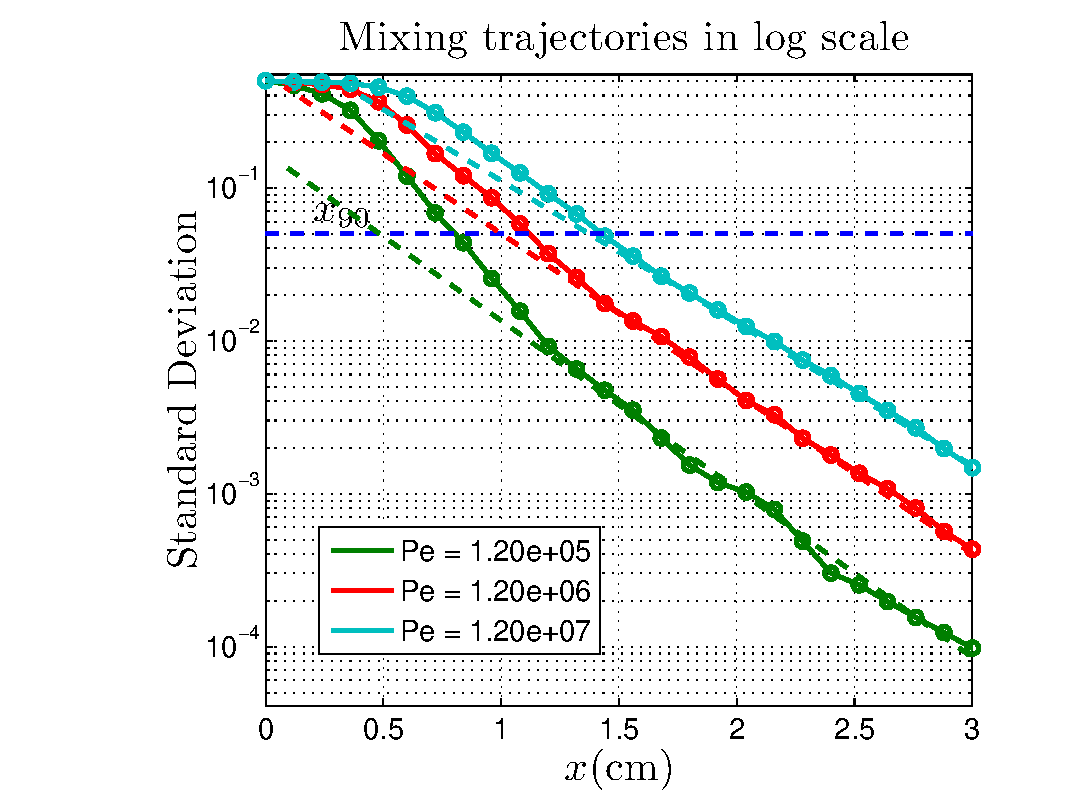
\includegraphics[width=0.7\textwidth]{example2veryPelog}
    \end{center}

\end{frame}

%%%%%%%%%%%%%%%%%%%%%%%%%%%%%%%%%%%%%%%%%%%%%%%%%%%%%%%%%%%%%%%%%%%%%%%
%%%%%%%%%%%%%%%%%%%%%%%%%%%%%%%%%%%%%%%%%%%%%%%%%%%%%%%%%%%%%%%%%%%%%%%
\begin{frame}
  \myframetitle{GSR Riffle Shuffles in Cards}
  \begin{itemize}
  \item Question: How many shuffles to randomize $52$ cards?
    \begin{center}
      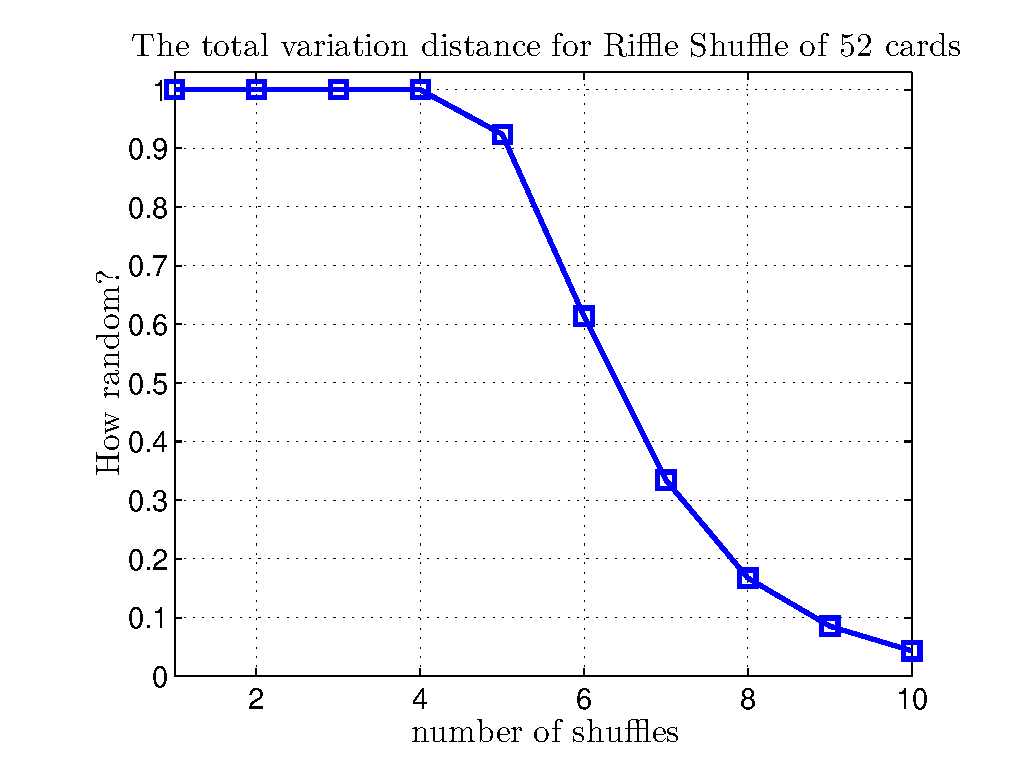
\includegraphics[width=0.55\textwidth,trim=1cm 1cm 0cm 0cm]{riffleshuffle}
    \end{center}
  \item Answer: 7.
  \item Aldous and Diaconis, 1986.
  \item A Markov Chain with $52! \approx 8 \times 10^{67}$ states.
  \end{itemize}
\end{frame}

%%%%%%%%%%%%%%%%%%%%%%%%%%%%%%%%%%%%%%%%%%%%%%%%%%%%%%%%%%%%%%%%%%%%%%%
%%%%%%%%%%%%%%%%%%%%%%%%%%%%%%%%%%%%%%%%%%%%%%%%%%%%%%%%%%%%%%%%%%%%%%%
\begin{frame}
\myframetitle{Cutoff in Finite Markov Chains}
    \begin{itemize}
     \item \textbf{Random walk on an $n$-dimensional hypercube} a particle starts at $\mathbf{0}$ and moves to one of its nearest neighbors (or stay fixed) with equal probability at each step.
     \item $(\Omega_n,\bar{\omega}_n, (\omega^k_n)_{k=0,1,...})_{n=1,2,...}$
    \end{itemize}
    \vspace{-0.2cm}
    \begin{center}
      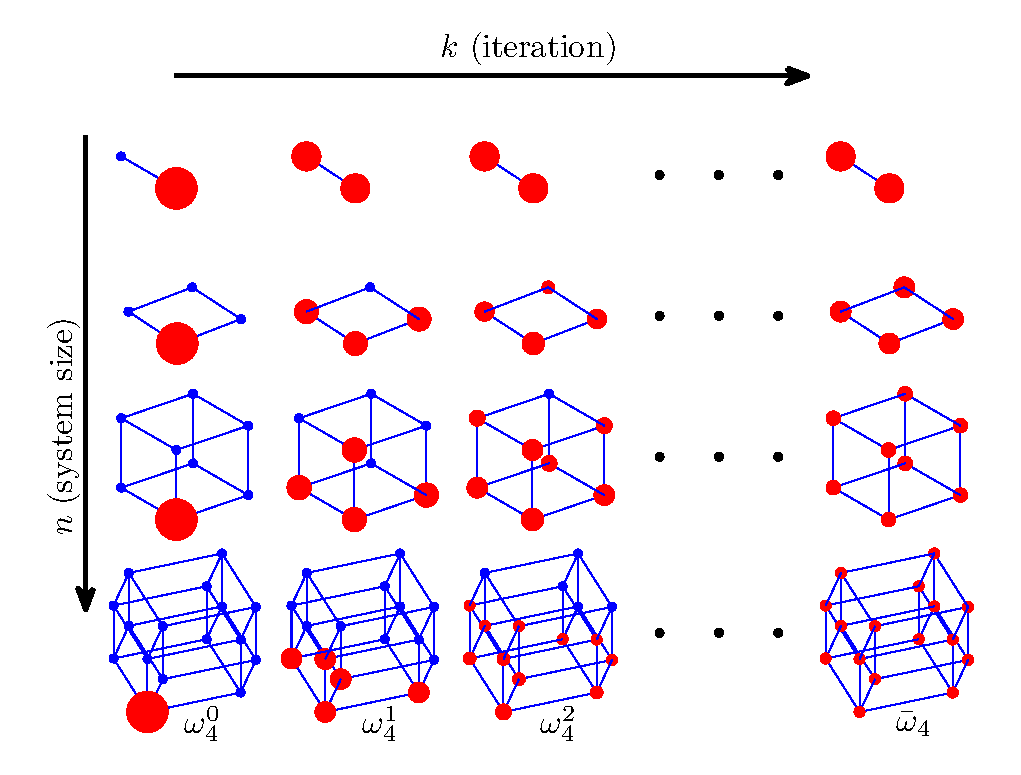
\includegraphics[width=0.58\textwidth]{cutoffdef}
    \end{center}
\end{frame}
%%%%%%%%%%%%%%%%%%%%%%%%%%%%%%%%%%%%%%%%%%%%%%%%%%%%%%%%%%%%%%%%%%%%%%%
%%%%%%%%%%%%%%%%%%%%%%%%%%%%%%%%%%%%%%%%%%%%%%%%%%%%%%%%%%%%%%%%%%%%%%%
\begin{frame}
  \myframetitle{Cutoff in Finite Markov Chains}
  \begin{itemize}
  \item Finite set $\Omega$ with ``metric'' $d$ on
    probability measures $\mu$, $\nu$, so that
    $d(\mu,\nu)$ such that 
    \begin{enumerate}
    \item $d(\mu,\nu)\in [0,1]$
    \item $\max_{\Omega,\mu,\nu} d(\mu,\nu) = 1$
    \item $d(\mu,\nu)=0$ if and only if $\mu=\nu$
    \end{enumerate}
  \item Sequence of probability spaces $(\Omega_n,\bar{\omega}_n)$,
    $n=1,2,\ldots$, each with a sequence of probability measures
    $\omega^k_n$, $k=0,1,\ldots$, such that
    \begin{align*}
      \lim_{k \rightarrow \infty} d(\omega^k_n,\bar{\omega}_n)=0
    \end{align*}
  \item Think of $n$ as dimension of a Markov Chain, $k$ as iteration
    number, $\omega^0_n$ as initial distribution, $\bar{\omega}_n$ as invariant
    distribution.
  \end{itemize}
\end{frame}
%%%%%%%%%%%%%%%%%%%%%%%%%%%%%%%%%%%%%%%%%%%%%%%%%%%%%%%%%%%%%%%%%%%%%%%
%%%%%%%%%%%%%%%%%%%%%%%%%%%%%%%%%%%%%%%%%%%%%%%%%%%%%%%%%%%%%%%%%%%%%%%
\begin{frame}
\myframetitle{Cutoff Phenomenon}
  \begin{itemize}
  \item Definition:\label{cutoffdefinition} (Diaconis) A family $(\Omega_n,\bar{\omega}_n, (\omega^k_n)_{k=0,1,...})_{n=1,2,...}$
   presents a D-cut-off if there exists a sequence $(t_n)$ of positive reals such that, for any $\epsilon \in(0,1)$,
  \begin{enumerate}
    \item $\lim_{n \rightarrow \infty}D(\omega^{k_n}_n,\bar{\omega}_n) = 0 \mbox{ if }
    k_n>(1+\epsilon)t_n$
    \item $\lim_{n \rightarrow \infty}D(\omega^{k_n}_n,\bar{\omega}_n) = 1 \mbox{ if }
    k_n<(1-\epsilon)t_n $
  \end{enumerate}
  \end{itemize}
\centerline{
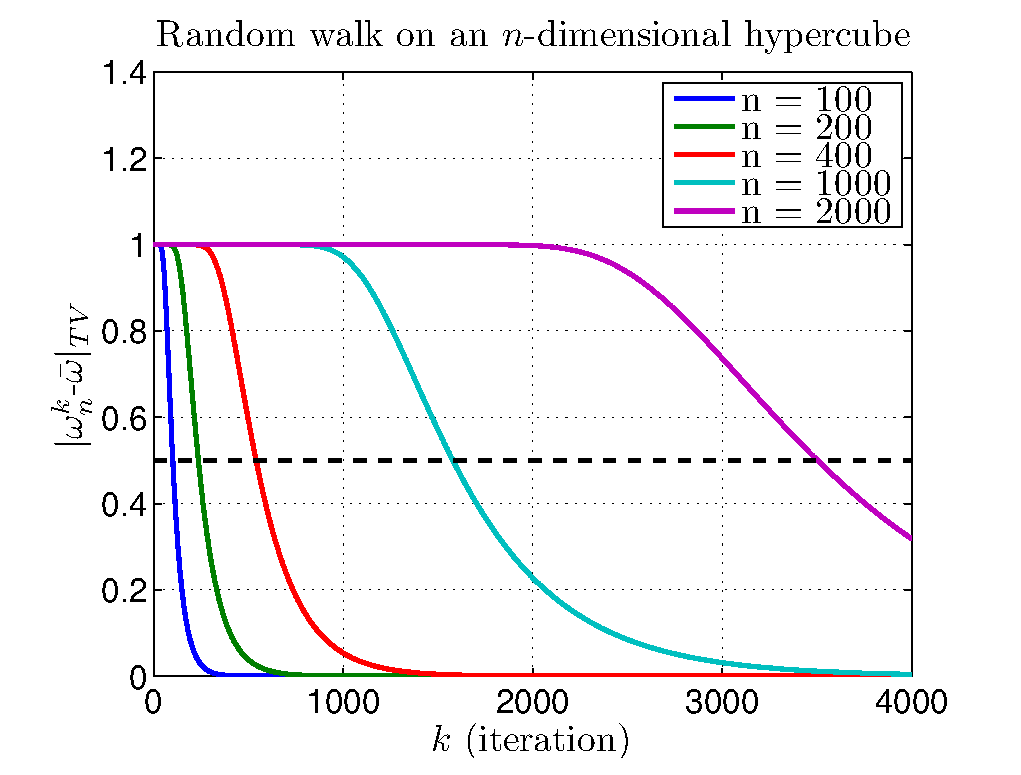
\includegraphics[width=0.43\textwidth,trim=1cm 1cm 0cm 0cm]{rdwalk}
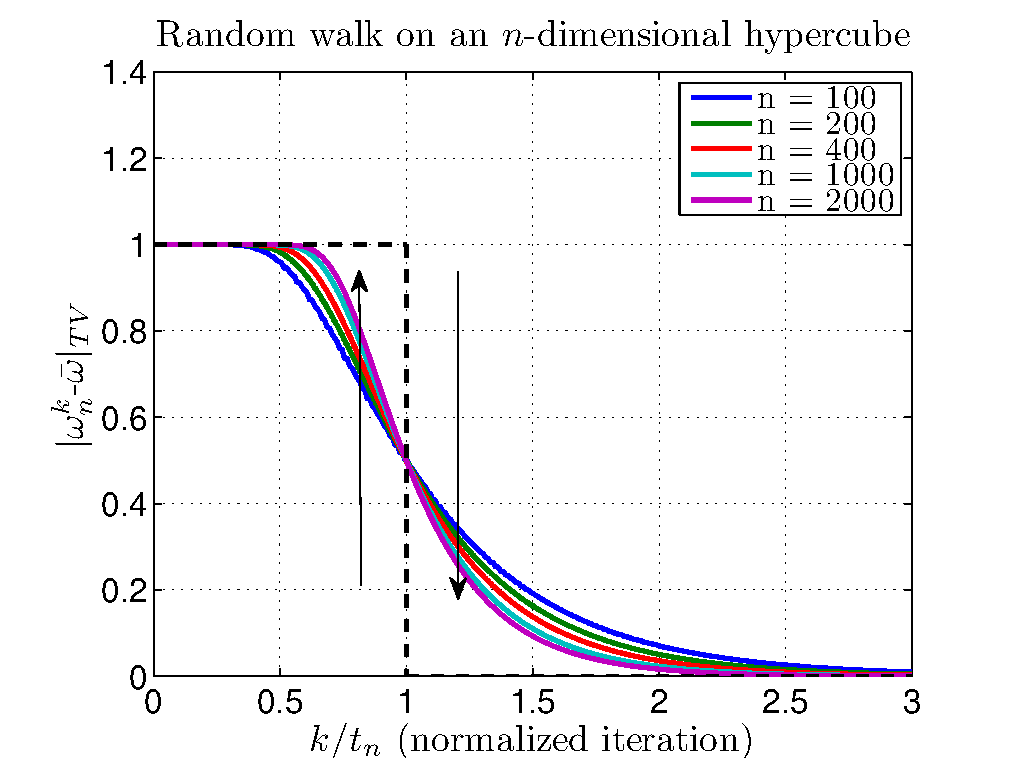
\includegraphics[width=0.43\textwidth,trim=1cm 1cm 0cm 0cm]{rdwalkn}
}


\end{frame}


%%%%%%%%%%%%%%%%%%%%%%%%%%%%%%%%%%%%%%%%%%%%%%%%%%%%%%%%%%%%%%%%%%%%%%%
%%%%%%%%%%%%%%%%%%%%%%%%%%%%%%%%%%%%%%%%%%%%%%%%%%%%%%%%%%%%%%%%%%%%%%%
\begin{frame}
\myframetitle{Cutoff Phenomenon}
  \begin{itemize}
  \item $\frac{\text{decay time}}{\text{cutoff time}} \rightarrow 0$ when $n \rightarrow \infty$. 
   \begin{center}
   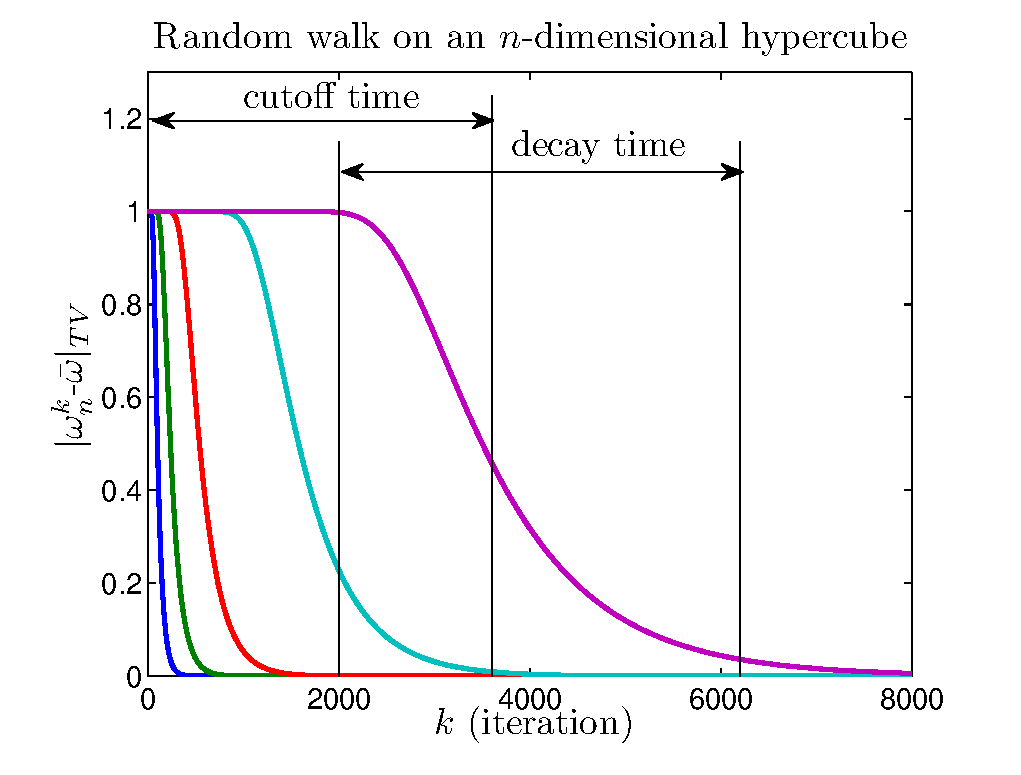
\includegraphics[width=0.43\textwidth,trim=1cm 1cm 0cm 0cm]{bntncutoff}
   \end{center}
  \vspace{0.2cm}
   \item ``To people studying finite Markov Chains, the fact theorem 3.1 (Riffle Shuffle Cutoff) can be proved at all appears like a miracle.'' - Laurent Saloff-Coste, Probability on Discrete Structures.
\end{itemize}
\end{frame}

%%%%%%%%%%%%%%%%%%%%%%%%%%%%%%%%%%%%%%%%%%%%%%%%%%%%%%%%%%%%%%%%%%%%%%%%
%%%%%%%%%%%%%%%%%%%%%%%%%%%%%%%%%%%%%%%%%%%%%%%%%%%%%%%%%%%%%%%%%%%%%%%%
\begin{frame}
\myframetitle{Evidence of Chaotic Map Cutoffs}
  \begin{itemize}
    \item Non-convex mixing long recognized in chaotic mixing literature.
      \begin{itemize}
       \item Super-exponential mixing phase.
      \end{itemize}
    \item Evidence of chaotic map cutoffs.
    \begin{itemize}
     \item $2$-D Baker's Map when diffusion goes to $0$.
     \item $2$-D Standard Map when diffusion goes to $0$.
     \item $1$-D Tent Map with a sequence of $w_n^0$.
     \item Any $1$-D chaotic map which symbolic dynamics.
    \end{itemize}
    \item Variance: $L_2$ cutoff, total variation distance: $L_1$ cutoff.
         \begin{itemize}
          \item Other mixing measures: $H^{-1}$ norm, mix-norm, etc. 
         \end{itemize}
    \item Evolving a distribution versus evolving a scalar function.
         \begin{itemize}
         \item $\int |\omega^k_n-\bar{\omega}_n| dx 
                = \int| \frac{\omega^k_n}{\bar{\omega}_n}-1|\bar{\omega}_n dx 
                = \int| f_n^k-1|\bar{\omega}_n dx $
         \end{itemize}
  \end{itemize}
\end{frame}

%%%%%%%%%%%%%%%%%%%%%%%%%%%%%%%%%%%%%%%%%%%%%%%%%%%%%%%%%%%%%%%%%%%%%%%
%%%%%%%%%%%%%%%%%%%%%%%%%%%%%%%%%%%%%%%%%%%%%%%%%%%%%%%%%%%%%%%%%%%%%%%
\begin{frame}
  \myframetitle{Cutoff in Baker's Map}
  \begin{itemize}
  \item Baker's map on $T^2$
    \begin{equation*}
      S(x_1,x_2) =
      \begin{cases}
        (2x_1,\frac{1}{2}x_2) \text{ mod } 1,
        & \text{if } 0 \le x_1 < \frac{1}{2} \\
        (2x_1,\frac{1}{2}(x_2+1)) \text{ mod } 1,
        & \text{if } \frac{1}{2} \le x_1 < 1
      \end{cases}
    \end{equation*}
  \item Initial condition $f^0(x)= \sqrt{\pi} \cos(2 \pi x_2)$
  \item Diffusion operator with diffusivity $D$ is applied after every
    iteration.
  \end{itemize}
  \begin{center}
    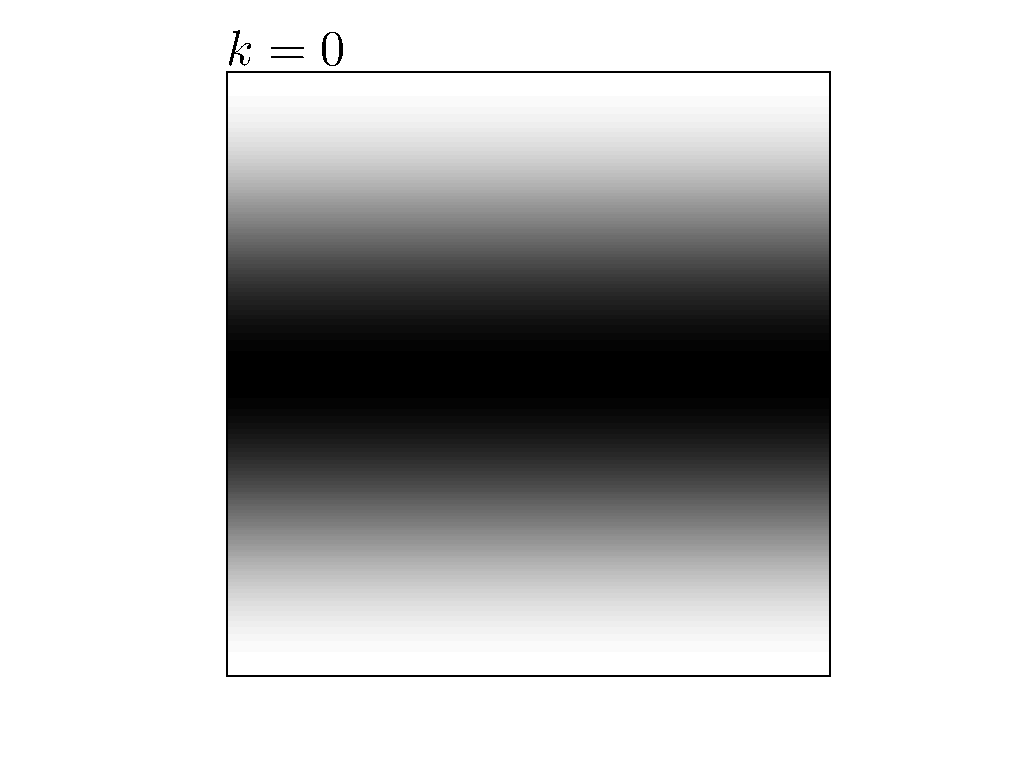
\includegraphics[width=0.3\textwidth,trim=1.2cm 1.2cm 1.2cm 1.2cm]{baker1}
    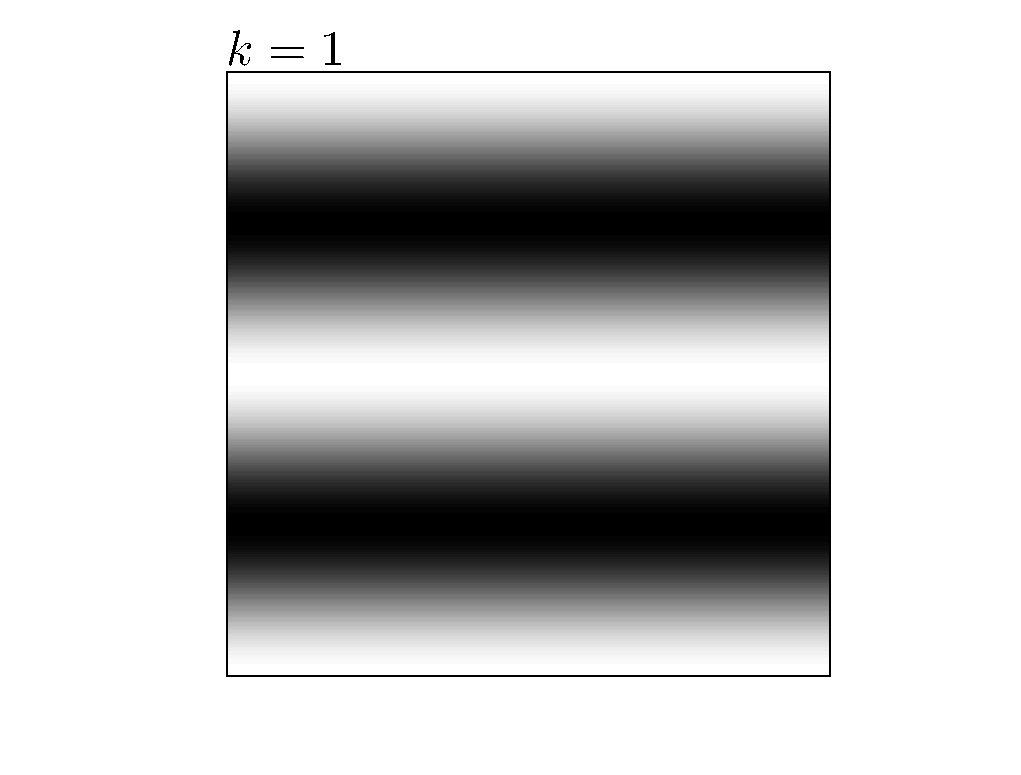
\includegraphics[width=0.3\textwidth,trim=1.2cm 1.2cm 1.2cm 1.2cm]{baker2}
    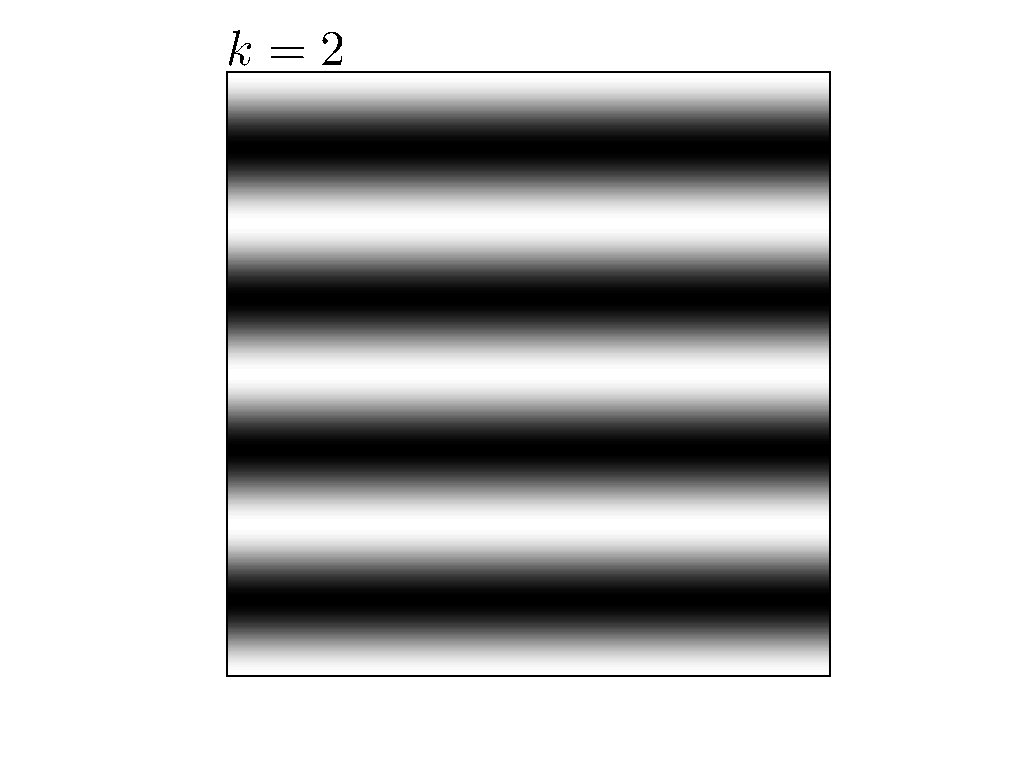
\includegraphics[width=0.3\textwidth,trim=1.2cm 1.2cm 1.2cm 1.2cm]{baker3}
  \end{center}
\end{frame}

%%%%%%%%%%%%%%%%%%%%%%%%%%%%%%%%%%%%%%%%%%%%%%%%%%%%%%%%%%%%%%%%%%%%%%%
%%%%%%%%%%%%%%%%%%%%%%%%%%%%%%%%%%%%%%%%%%%%%%%%%%%%%%%%%%%%%%%%%%%%%%%
\begin{frame}
  \myframetitle{Cutoff in Baker's Map}
  \begin{itemize}
  \item Analytically solvable:
    \begin{align*}
      f^k(x) &= \sqrt{\pi} e^{-4 \pi^2 D 2 ^{2 k}}\cos(2 \pi 2^k x_2)
      \text{ for } k = 1,2,\ldots \\
      \text{var}(f^k(x)) &= e^{-8 \pi^2 D 2^{2 k}}
    \end{align*}
  \item Cutoff time: $t_n \sim -\log(D).$
    \begin{center}
      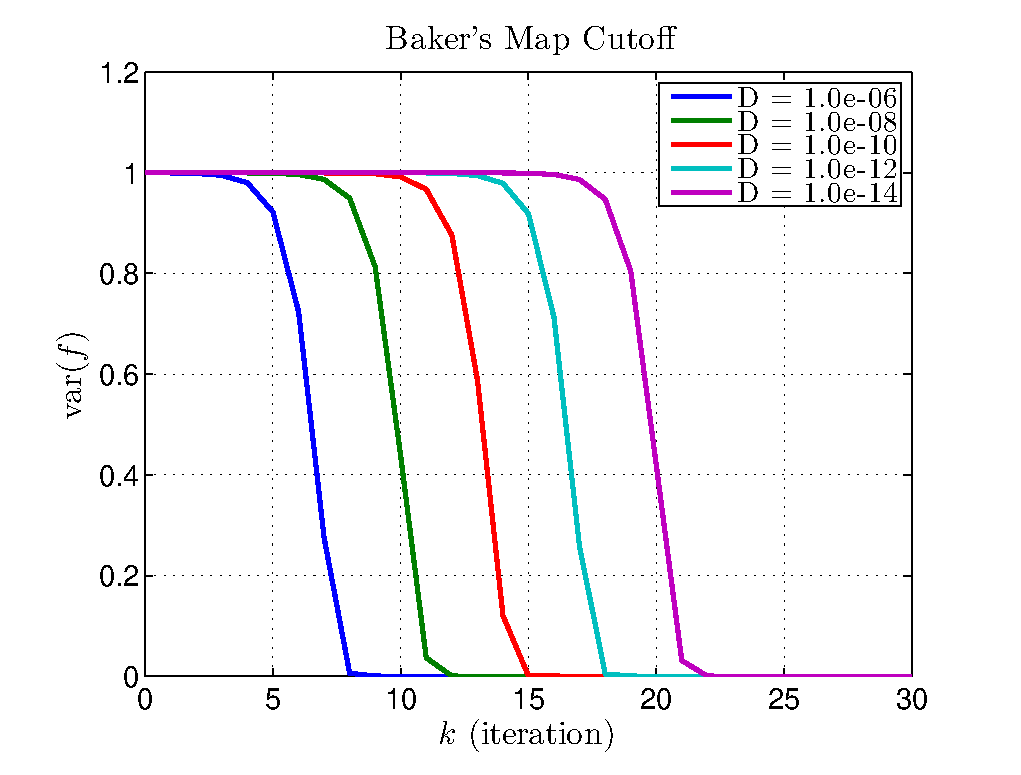
\includegraphics[width=0.54\textwidth]{bakersmapcutoff}
      %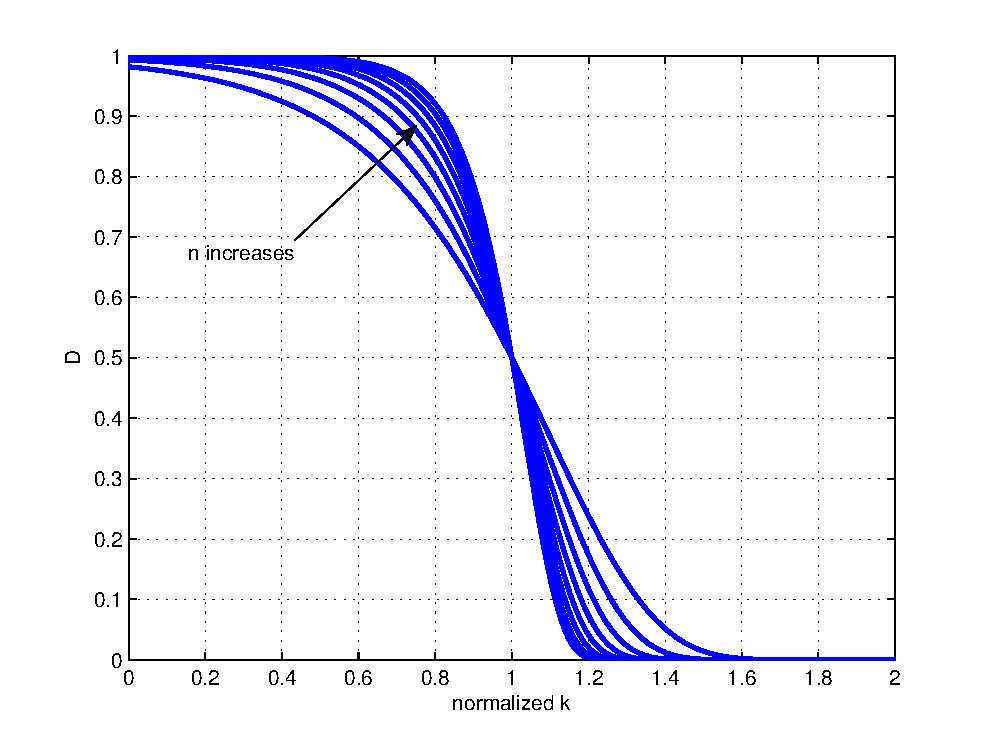
\includegraphics[width=5cm]{democutoff1n}
    \end{center}
  \end{itemize}
\end{frame}
%%%%%%%%%%%%%%%%%%%%%%%%%%%%%%%%%%%%%%%%%%%%%%%%%%%%%%%%%%%%%%%%%%%%%%%
%%%%%%%%%%%%%%%%%%%%%%%%%%%%%%%%%%%%%%%%%%%%%%%%%%%%%%%%%%%%%%%%%%%%%%%
\begin{frame}
\myframetitle{Standard Map}

\centerline{
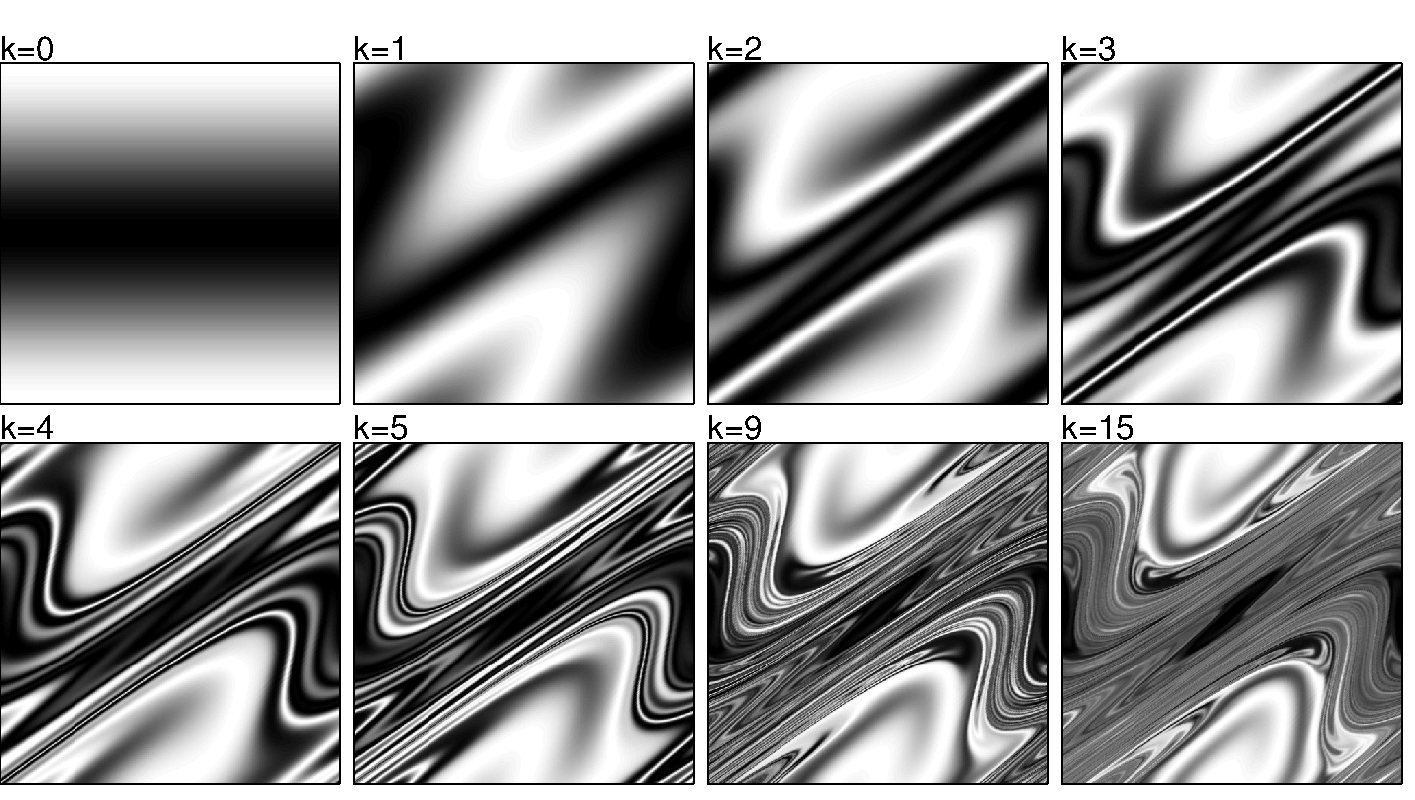
\includegraphics[width=0.75\textwidth,trim=1cm 1cm 0cm 0cm]{standardmapevolve}
}
   \begin{align*}
   \\[-1cm]
     \begin{cases}
        x_1 \leftarrow x_1+x_2 +\epsilon \sin{2 \pi x_1}  \mbox{ (mod } 1)\\
        x_2 \leftarrow  x_2 +\epsilon \sin{2 \pi x_1}     \mbox{ (mod } 1)
     \end{cases}
   \end{align*}
   \begin{equation*}
      \epsilon=0.3, \,\, f^0   = \cos(2\pi x_2)
   \end{equation*}

\end{frame}

%%%%%%%%%%%%%%%%%%%%%%%%%%%%%%%%%%%%%%%%%%%%%%%%%%%%%%%%%%%%%%%%%%%%%%%
%%%%%%%%%%%%%%%%%%%%%%%%%%%%%%%%%%%%%%%%%%%%%%%%%%%%%%%%%%%%%%%%%%%%%%%
\begin{frame}
\myframetitle{Standard Map Cutoff?} 
\begin{center}
    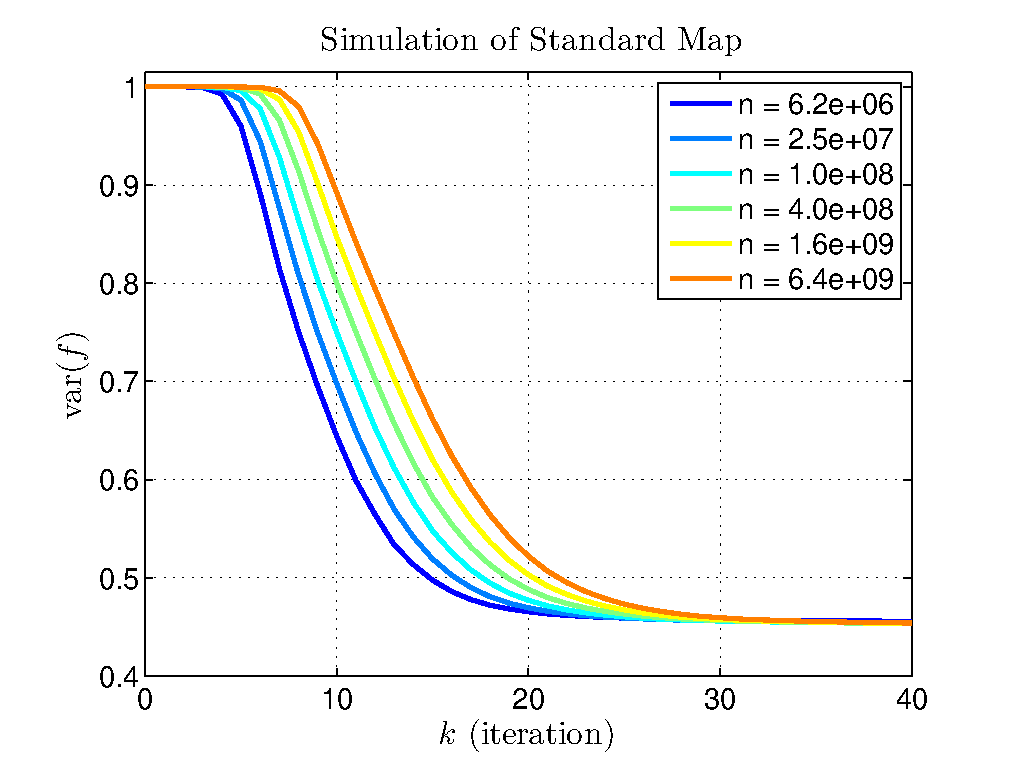
\includegraphics[width=0.45\textwidth,trim=1cm 1cm 0cm 0cm]{standardmapcutoff2}
    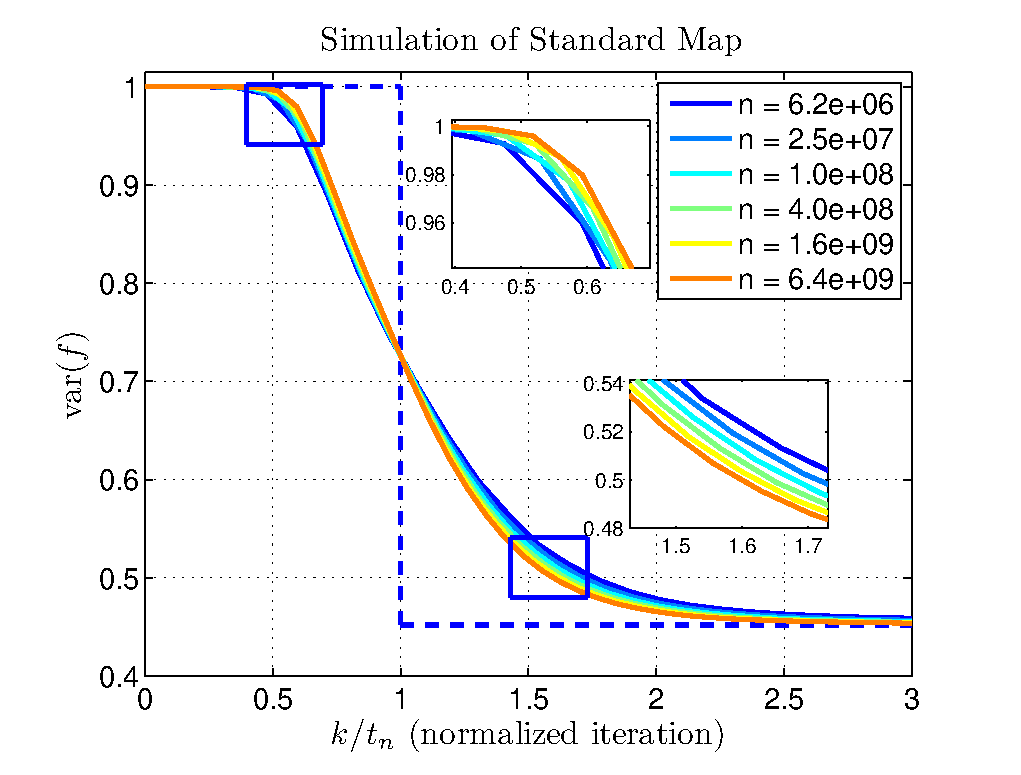
\includegraphics[width=0.45\textwidth,trim=1cm 1cm 0cm 0cm]{standardmapcutoffn2}
\end{center}
  \begin{itemize}
    \item Standard map, $\epsilon = 0.3$, $f^0 = \cos(2\pi x_2)$.
    \item $(M,m) = (1,0.4521)$.
    \item Cutoff time: $t_n =\min \{ k \mid \text{var}(f^k_n)< \frac{M+m}{2}\}. $
    \item Only looks slow because we can't simulate large systems($6.4\times 10^9$ already! but riffle shuffle has $8 \times 10^{67}$).
\end{itemize}

\end{frame}

%%%%%%%%%%%%%%%%%%%%%%%%%%%%%%%%%%%%%%%%%%%%%%%%%%%%%%%%%%%%%%%%%%%%%%%
%%%%%%%%%%%%%%%%%%%%%%%%%%%%%%%%%%%%%%%%%%%%%%%%%%%%%%%%%%%%%%%%%%%%%%%
\begin{frame}
\myframetitle{Numerical Evidence of Standard Map Cutoff}
   \begin{center}
    %\begin{tabular}{rl}
     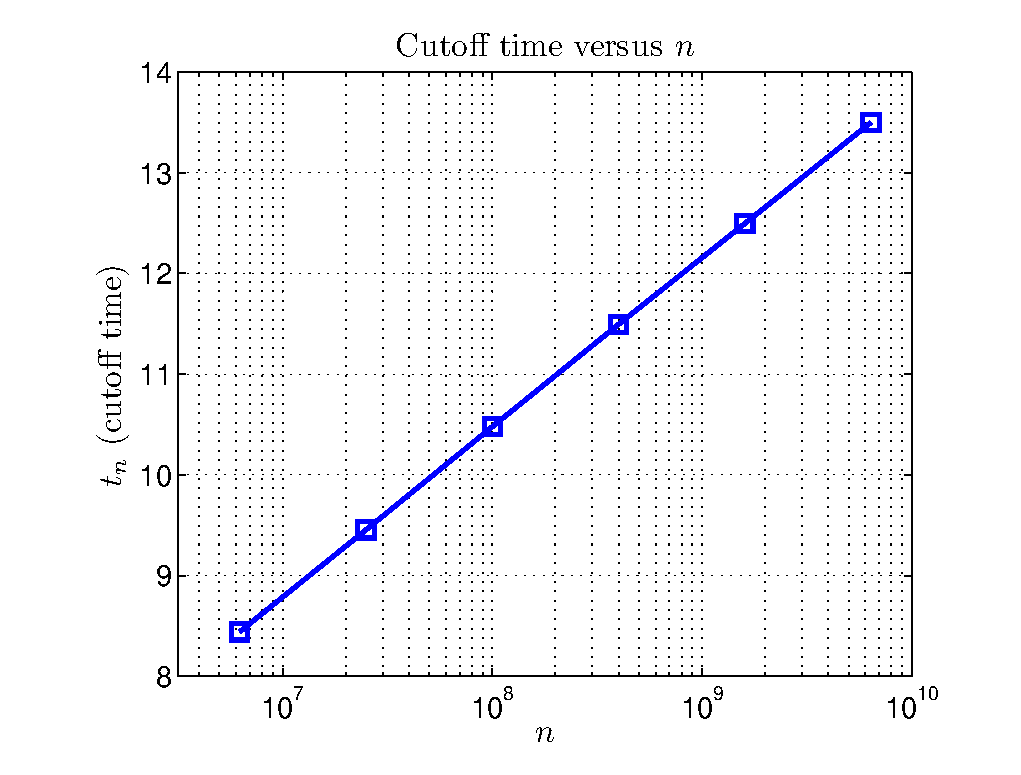
\includegraphics[width=0.45\textwidth,trim=1cm 1cm 0cm 0cm]{cutofftimevsD2}
     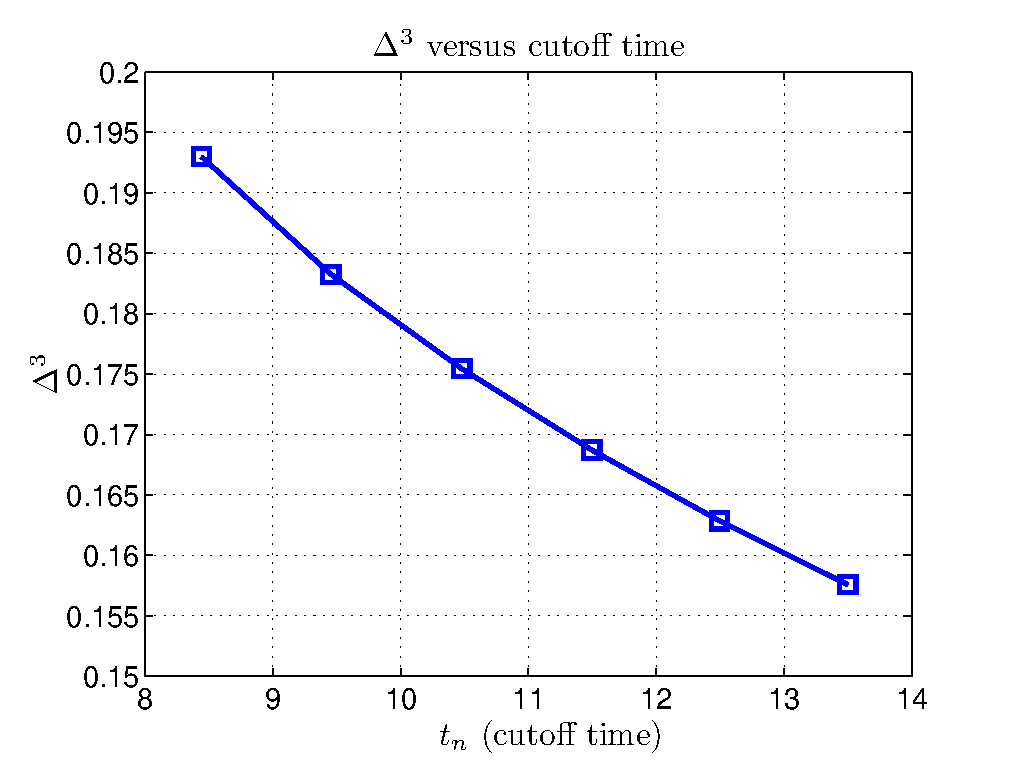
\includegraphics[width=0.45\textwidth,trim=1cm 1cm 0cm 0cm]{areavscutofftime2}
    %\end{tabular}
   \end{center}
    \begin{itemize}
    \item $t_n \sim \log(n) \sim -\log(D)$
    \item Measure distance to step transition:
     \begin{equation*}
       c^{\infty}(x) = \begin{cases}
         M, &\text{if } x < 1, \\
         m, &\text{otherwise}
       \end{cases}
      \qquad
      \Delta^l = \int_0^l | c^k(x)-c^{\infty}(x)|\,dx
    \end{equation*}
  \end{itemize}

\end{frame}
%%%%%%%%%%%%%%%%%%%%%%%%%%%%%%%%%%%%%%%%%%%%%%%%%%%%%%%%%%%%%%%%%%%%%%%
%%%%%%%%%%%%%%%%%%%%%%%%%%%%%%%%%%%%%%%%%%%%%%%%%%%%%%%%%%%%%%%%%%%%%%%
%\begin{frame}
%\myframetitle{Tent Map ``Cutoff''}
%\begin{center}
%\vspace{-0.4cm}
%\begin{tabular}{rcl}
%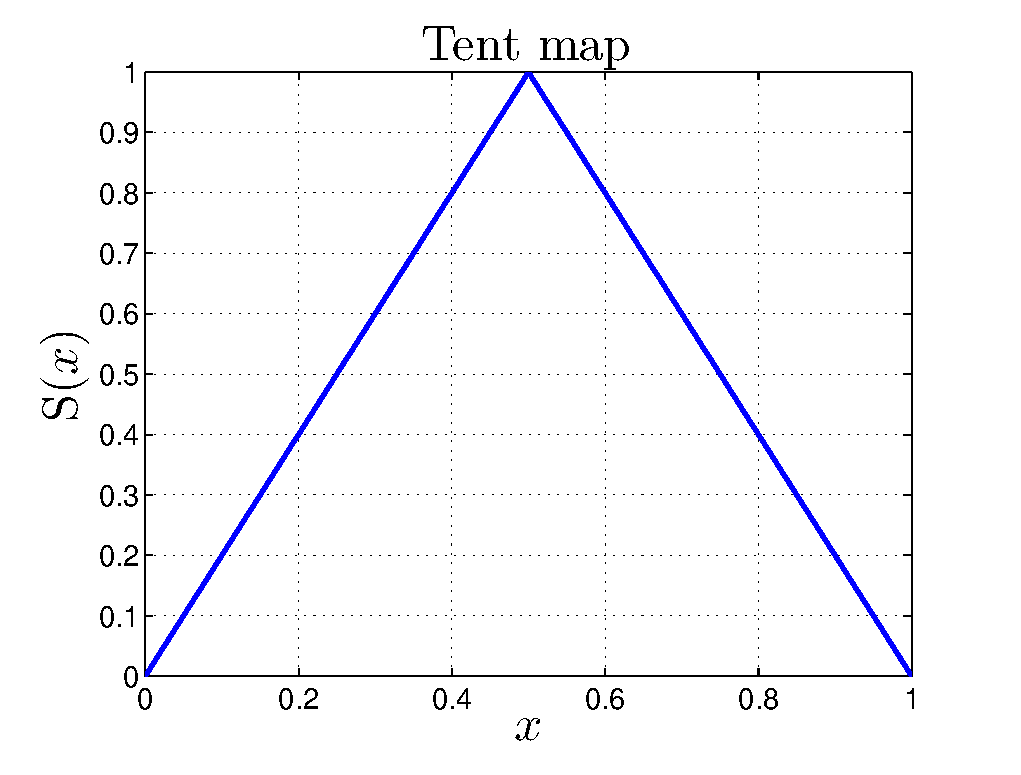
\includegraphics[height=2.7cm,trim=1cm 1cm 1cm 1cm]{tentmap}&
%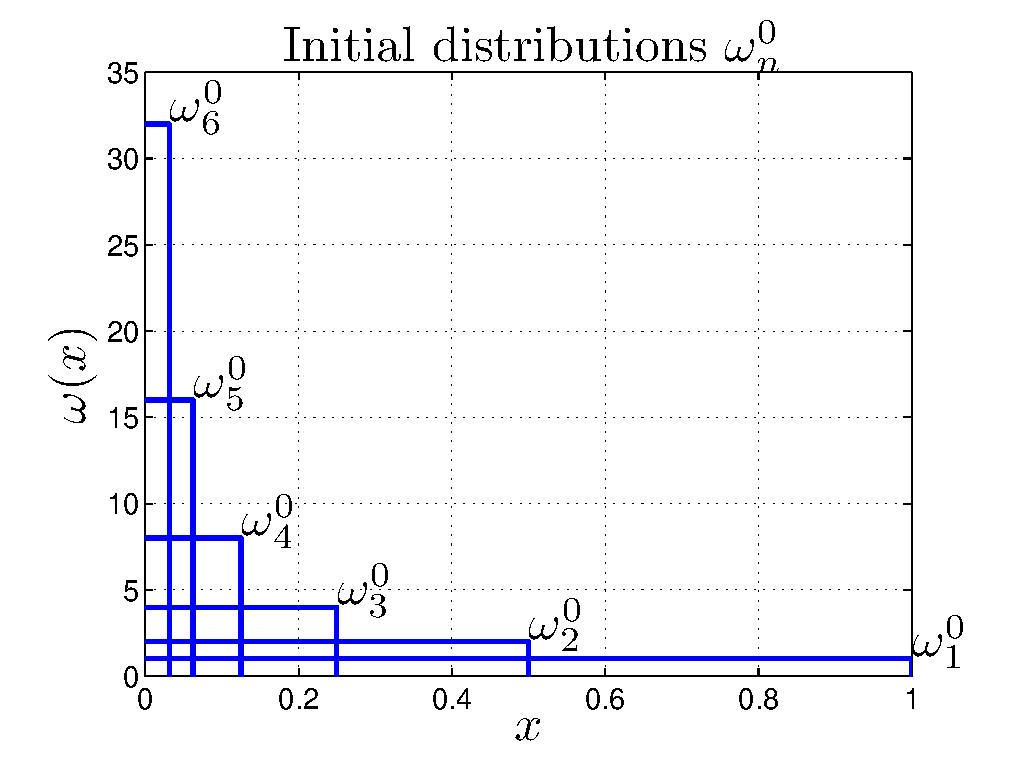
\includegraphics[height=2.7cm,trim=1cm 1cm 1cm 1cm]{tentmapomega0}&
%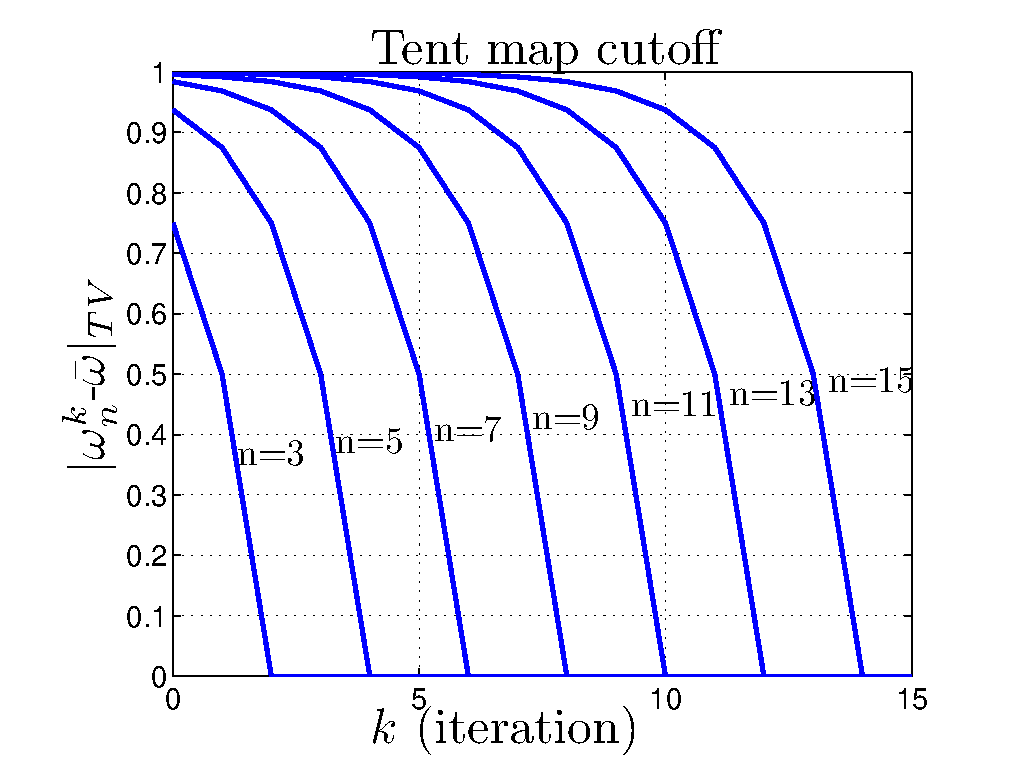
\includegraphics[height=2.7cm,trim=1cm 1cm 1cm 1cm]{tentmapcutoff}
%\end{tabular}
%\vspace{-0.3cm}
%\end{center}
%   \begin{eqnarray}
%   \label{tentmap}
%     x \leftarrow S_\text{tent}(x) \equiv 1-2\left|x-\frac{1}{2}\right|,\
%     P_S(\omega_n^k(x)) = \frac{1}{2}\left(\omega_n^k\left(\frac{x}{2}\right)+\omega_n^k\left(1-\frac{x}{2}\right) \right)\nonumber
%   \end{eqnarray}
%with the following initial distributions on $[0 ,1]$,
%  \begin{eqnarray}
%  \label{tentmapinitial}
%    \omega_n^0 = \left\{ \begin{tabular}{c}
%                      $\frac{1}{\mu_n}$, \mbox{  if  } $x \le \mu_n$\\
%                      $0$, \mbox{  otherwise}
%                      \end{tabular}\right.
%  \end{eqnarray}
%where $\mu_1 = 1$, and $\mu_{n+1} = \frac{\mu_n}{2}$.
%\end{frame}

%%%%%%%%%%%%%%%%%%%%%%%%%%%%%%%%%%%%%%%%%%%%%%%%%%%%%%%%%%%%%%%%%%%%%%%
%%%%%%%%%%%%%%%%%%%%%%%%%%%%%%%%%%%%%%%%%%%%%%%%%%%%%%%%%%%%%%%%%%%%%%%
\begin{frame}
\myframetitle{Tent Map Cutoff}
\begin{center}
\vspace{-0.4cm}
\begin{tabular}{rcl}
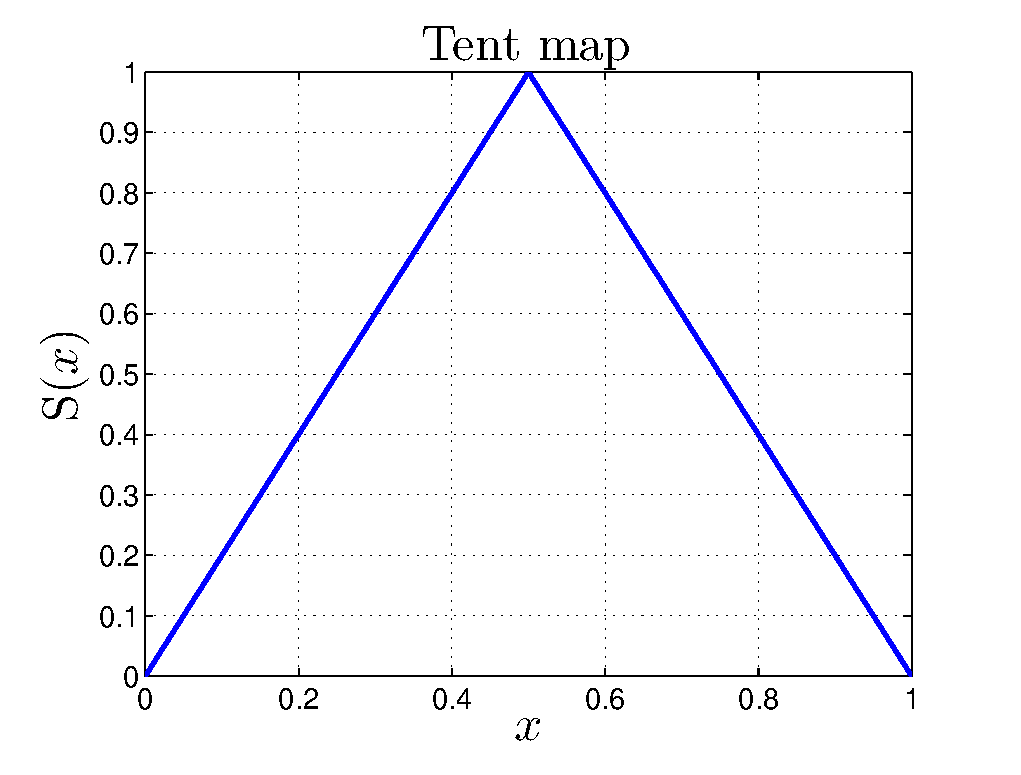
\includegraphics[height=2.7cm,trim=1.5cm 0.7cm 1cm 1cm]{tentmap}&
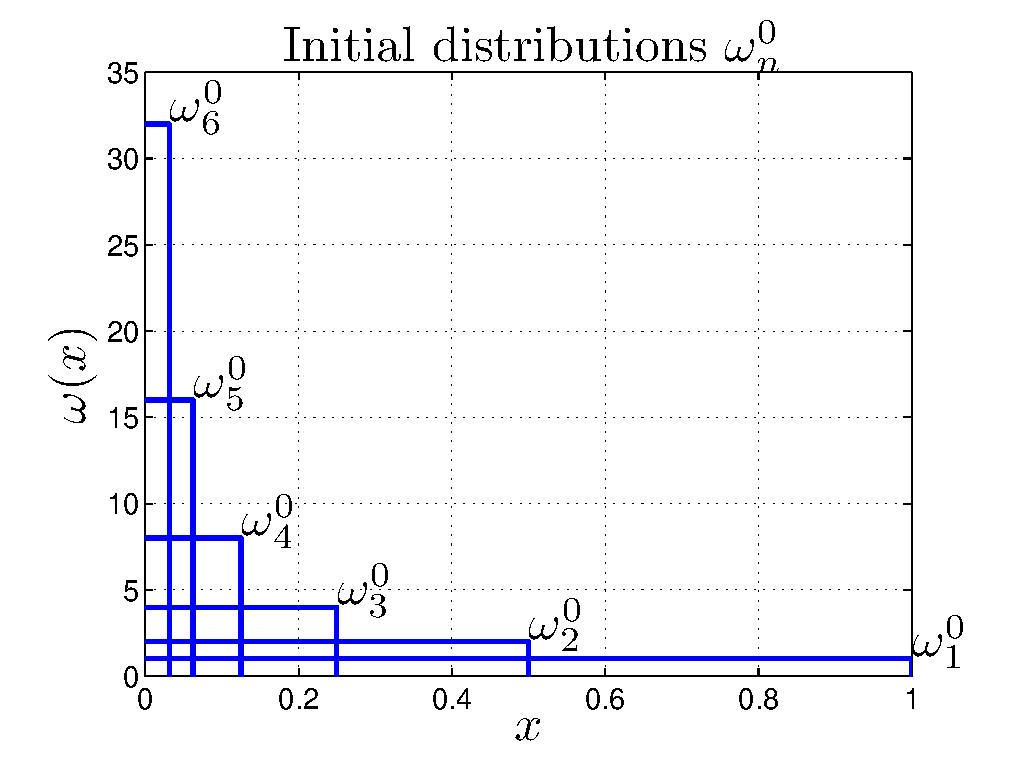
\includegraphics[height=2.7cm,trim=1.1cm 0.7cm 1cm 1cm]{tentmapomega0}&
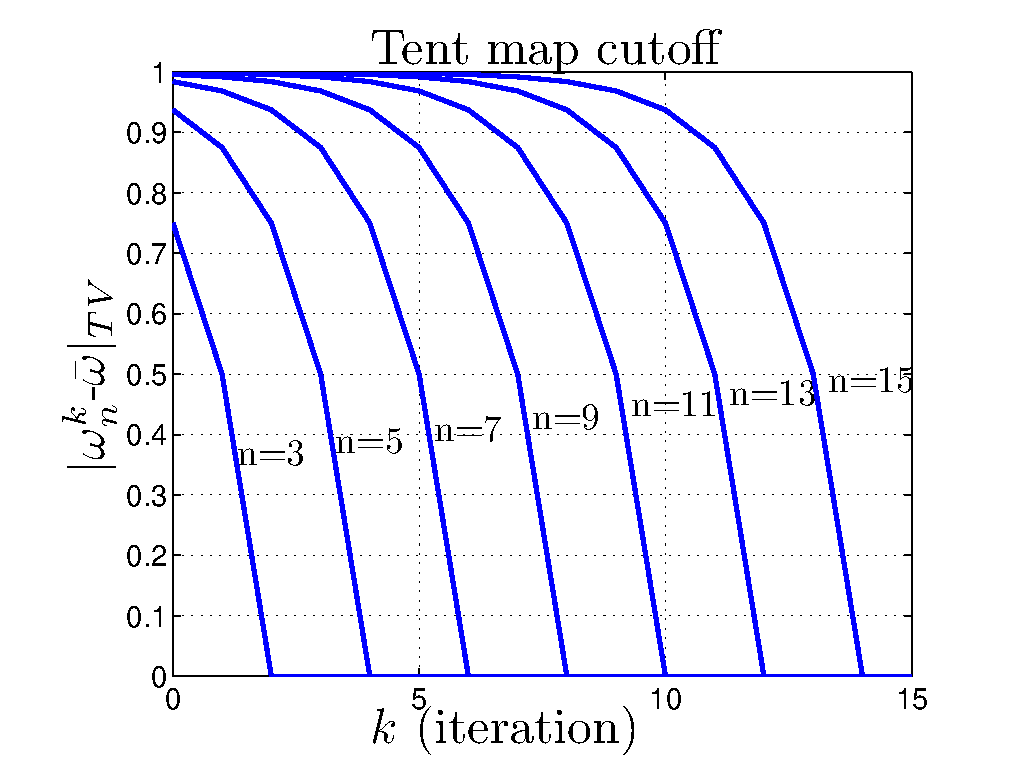
\includegraphics[height=2.7cm,trim=1.1cm 0.7cm 1cm 1cm]{tentmapcutoff}
\end{tabular}
\vspace{-0.3cm}
\end{center}
\begin{itemize}
  \item Tent map: $x \leftarrow S_\text{tent}(x) = 1-2\left|x-\frac{1}{2}\right|$
  \item $P_S(\omega_n^k(x)) = \frac{1}{2}\left(\omega_n^k\left(\frac{x}{2}\right)+\omega_n^k\left(1-\frac{x}{2}\right) \right)$
  \item Not volume-preserving.  
     \begin{itemize}
      \item Initial distribution $\omega_n^0$ is a sequence of square functions converging to a delta function.
  \begin{eqnarray*}
  \label{tentmapinitial}
    \omega_n^0 = \left\{ \begin{tabular}{c}
                      $\frac{1}{\mu_n}$, \mbox{  if  } $x \le \mu_n$\\
                      $0$, \mbox{  otherwise}
                      \end{tabular}\right.
  \end{eqnarray*}
where $\mu_1 = 1$, and $\mu_{n+1} = \frac{\mu_n}{2}$.
     \end{itemize}
\end{itemize}
\end{frame}

%%%%%%%%%%%%%%%%%%%%%%%%%%%%%%%%%%%%%%%%%%%%%%%%%%%%%%%%%%%%%%%%%%%%%%%
%%%%%%%%%%%%%%%%%%%%%%%%%%%%%%%%%%%%%%%%%%%%%%%%%%%%%%%%%%%%%%%%%%%%%%%
\begin{frame}
 \myframetitle{Create Cutoffs from Symbolic Dynamics}
\begin{theorem}
Given a $1$-D chaotic map with symbolic dynamics, there exists (and we can construct) a sequence $\omega_n^0$ such that the family
$(\Omega,\bar{\omega},(\omega^k_n)_{k=0,1,...})_{n=1,2,...}$ presents a Total Variation-cutoff. In fact, let $k =
\frac{1}{4}n\log{n}+cn $ for $c\in \mathbb{R}$. As $n\rightarrow \infty$,
\begin{eqnarray*}
\label{erfbound}
 %|\omega^k_n - \bar{\omega} |_{TV} \sim \erf \left(\frac{e^{-2c}}{\sqrt{8}}\right)
       |\omega^k_n - \bar{\omega} |_{TV} \sim \erf \left(\frac{e^{-2c}}{\sqrt{8}}\right)
\end{eqnarray*}
\end{theorem}

 (Diaconis 1990) For the random walk on an $n$-dimensional hypercube problem, let $k = \frac{1}{4}n\log{n}+cn$ for $c \in \mathbb{R}$. As $n \rightarrow \infty$,
\begin{eqnarray*}
\label{rdwalkshape}
 |\omega^k_n - \bar{\omega} |_{TV} \sim \erf\left(\frac{e^{-2c}}{\sqrt{8}}\right)
\end{eqnarray*}
\end{frame}

%%%%%%%%%%%%%%%%%%%%%%%%%%%%%%%%%%%%%%%%%%%%%%%%%%%%%%%%%%%%%%%%%%%%%%%
%%%%%%%%%%%%%%%%%%%%%%%%%%%%%%%%%%%%%%%%%%%%%%%%%%%%%%%%%%%%%%%%%%%%%%%
\begin{frame}
 \myframetitle{Idea of Proof}
\begin{itemize}
   \item Claim: The process is composed of many (almost) independent processes $\Longrightarrow$ cutoff.
   \item Random walk on an $n$-dimensional hypercube problem,
         \begin{align*}
          x^0 = (0,0,0,0,0,0,0,...)
          \end{align*}
         Each of the coordinates equals $0$ with probability $1$ initially.
   \item $\prob(x^k_i=0)$ and $\prob(x^k_j=0)$, $i \neq j$ are not independent.
   \item When $k$ is large, $\prob(x^k_i=0)$ converges to $\frac{1}{2}$ almost independently for all $i$.
   \item $\prob(x^k_i=0) = \frac{1}{2}+\frac{1}{2}\left(\frac{n-1}{n+1}\right)^k $
   \item $\lambda_2 = \frac{n-1}{n+1}$ with multiplicity $n$.

    %\begin{center}
    %      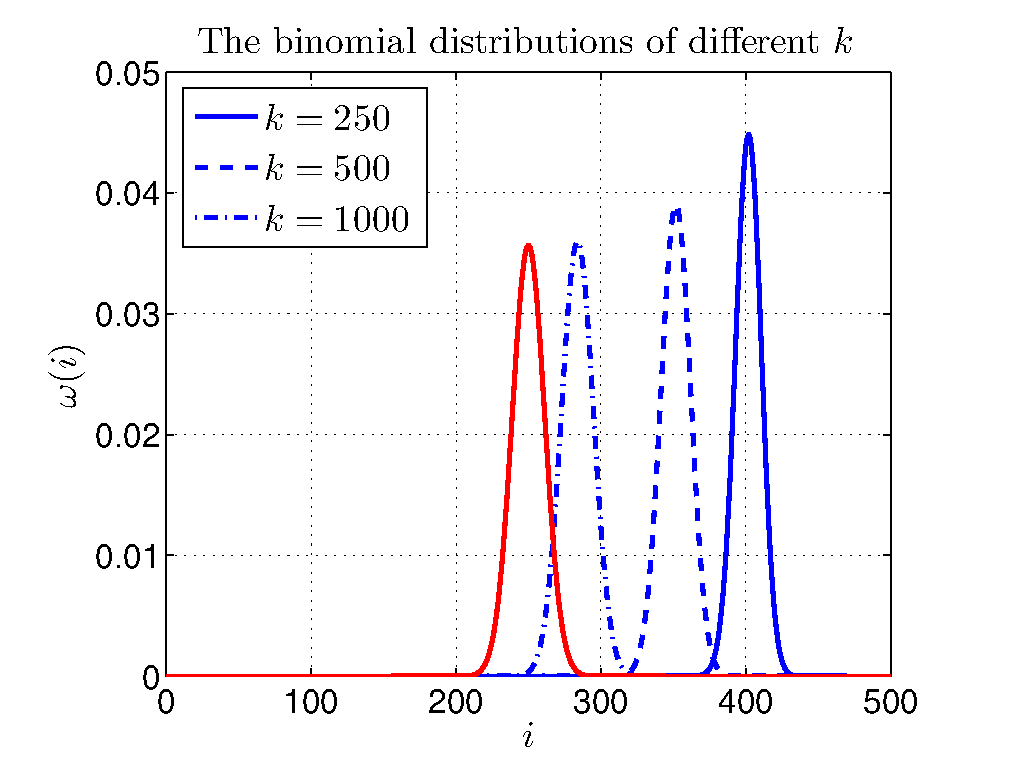
\includegraphics[height=2.7cm,trim=1cm 1cm 1cm 1cm]{deltaMexample2a}
    %      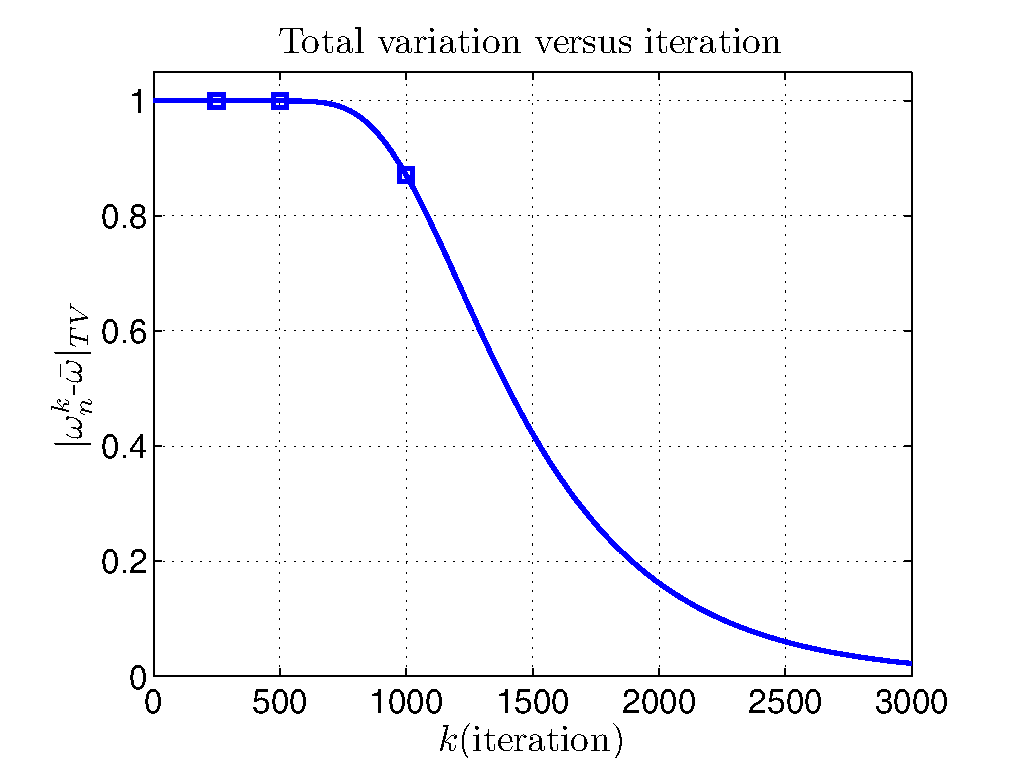
\includegraphics[height=2.7cm,trim=1cm 1cm 1cm 1cm]{ehrenfasttv}
    %\end{center}

\end{itemize}

\end{frame}
%%%%%%%%%%%%%%%%%%%%%%%%%%%%%%%%%%%%%%%%%%%%%%%%%%%%%%%%%%%%%%%%%%%%%%%
%%%%%%%%%%%%%%%%%%%%%%%%%%%%%%%%%%%%%%%%%%%%%%%%%%%%%%%%%%%%%%%%%%%%%%%
%\begin{frame}
% \myframetitle{Idea of Proof: Symbolic Dynamics}
%  \begin{center}
%          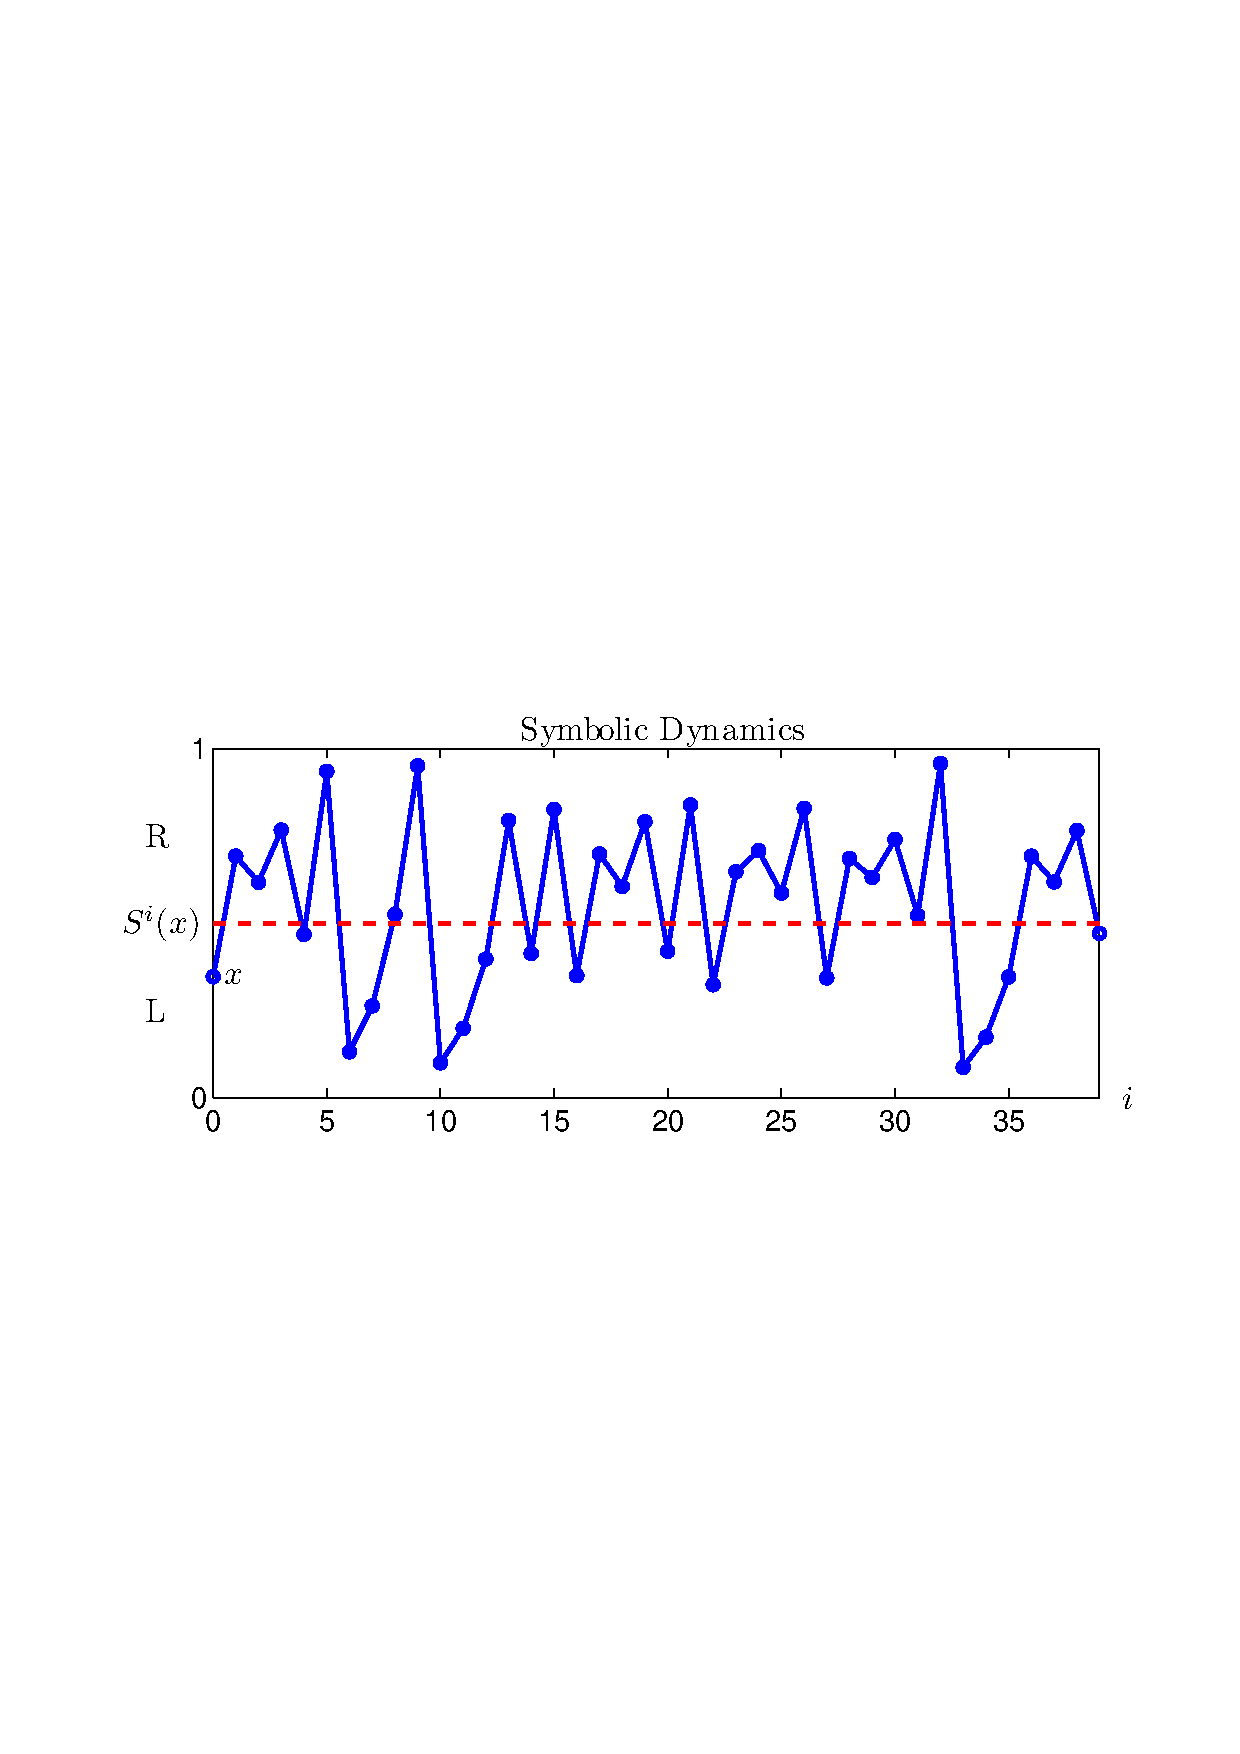
\includegraphics[height=2.7cm,trim=1cm 1cm 1cm 1cm]{symbolicdynamics_edit}
%  \end{center}
%  \begin{itemize}
%     \item $S(x): [0, 1] \rightarrow [0, 1]$ is a chaotic map.
%     \item For a deterministic $x$, $\phi: x \mapsto \{s_0s_1s_2...\} = \{LRRRLR...\}. $
%     \item For a probabilistic distribution $\omega$, $\psi: \omega  \mapsto \{\delta_0\delta_1\delta_2...\}$, $\delta_i\in[0,1]$, $\delta_i=\prob(s_i=L)$.
%     \item There exists a subspace $\bar{\Omega}$, such that if $\omega \in \bar{\Omega}$, $s_0,s_1,s_2,...$ are all independent.

%  \end{itemize}
%\end{frame}

\begin{frame}
  \myframetitle{Stochastic Symbolic Dynamics}
  \begin{center}
    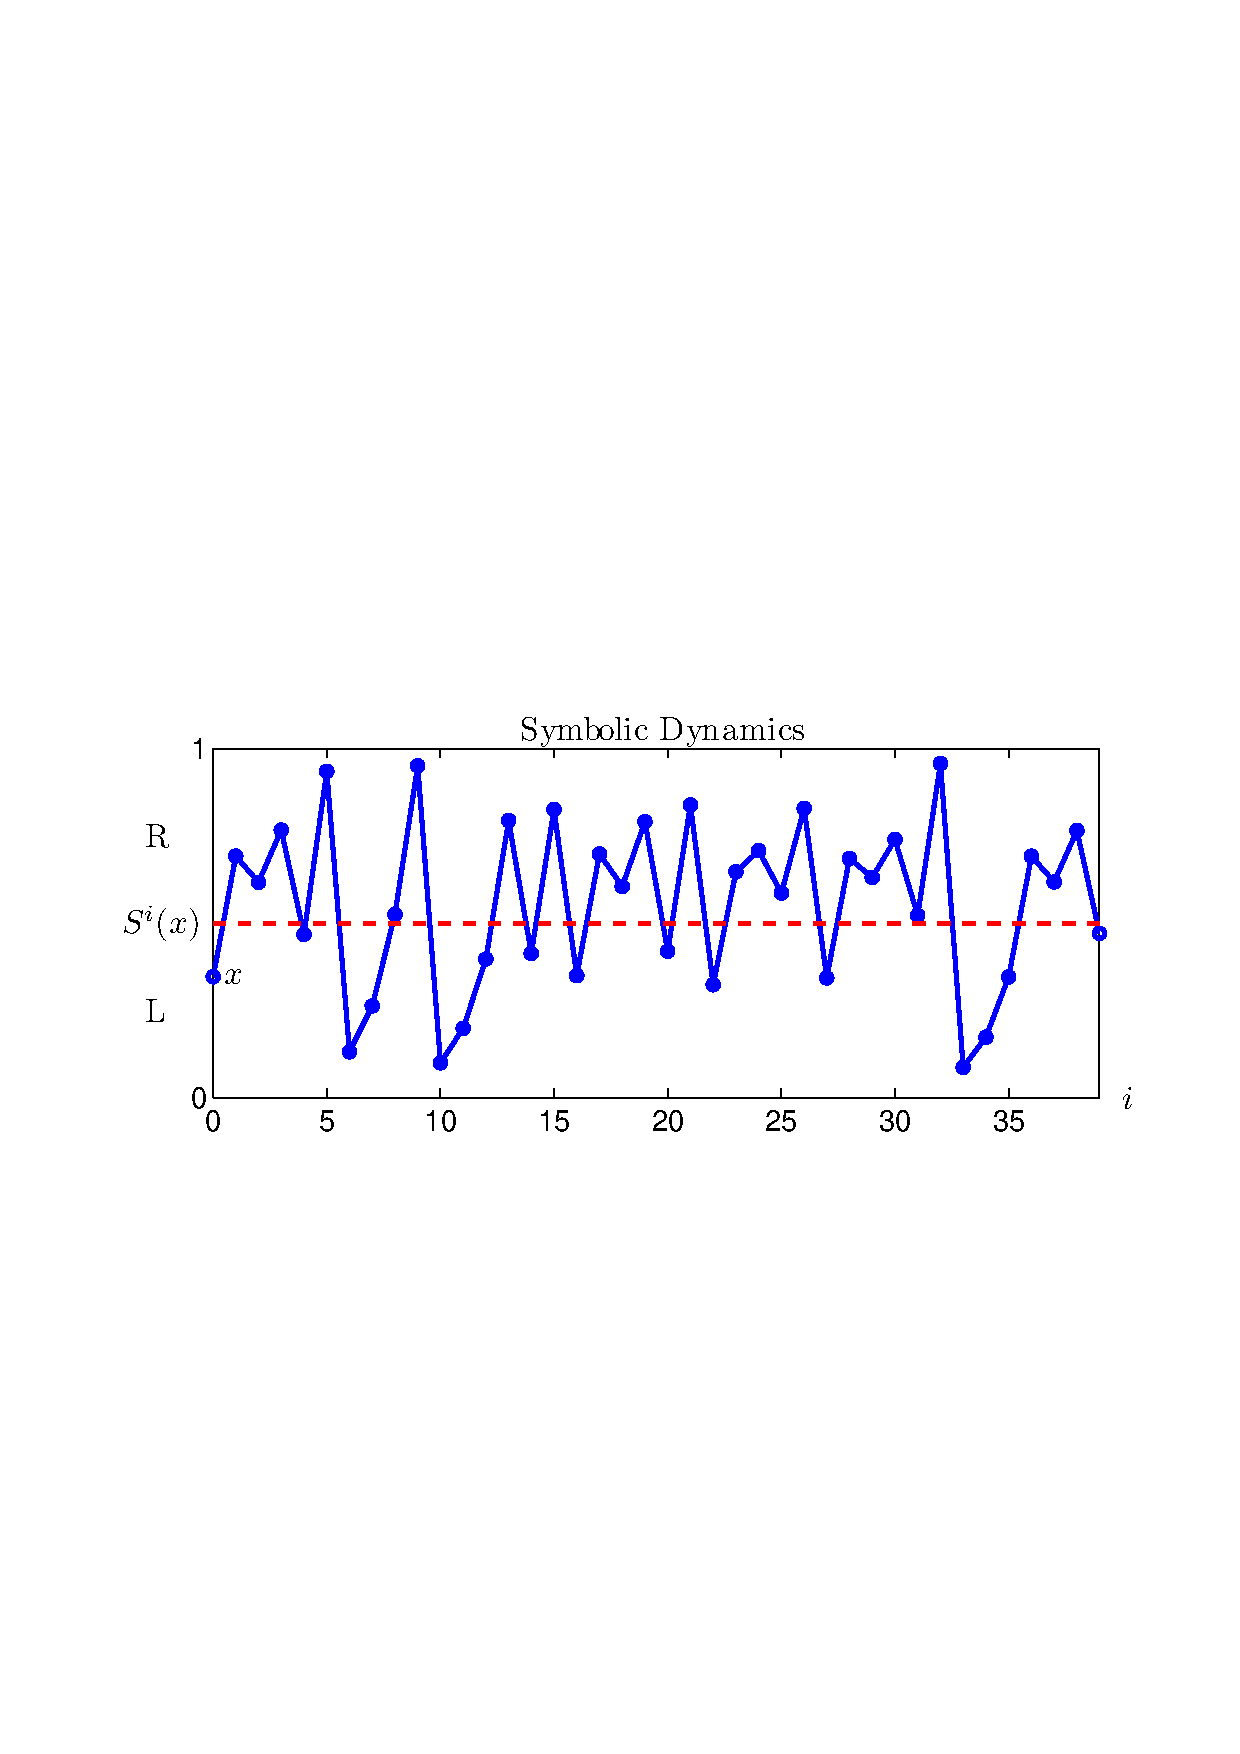
\includegraphics[height=2.5cm,trim=1cm 1cm 1cm 1cm]{symbolicdynamics_edit}
  \end{center}
  \begin{itemize}
  \item Extend to stochastic symbolic dynamics:
    \begin{itemize}
    \item $S(x): [0, 1] \rightarrow [0, 1]$ is a chaotic map.
    \item For a deterministic $x$, $\phi: x \mapsto \{s_0s_1s_2...\} =
      \{LRRRLR...\} $.
    \item $S$ and a shift operator are topologically conjugate.  
    \item For a probabilistic distribution $\omega$, $\psi: \omega
      \mapsto \{\delta_0\delta_1\delta_2...\}$, 
      $\delta_i=\operatorname*{Prob}(s_i=L) \in [0,1]$
        \item There exists a subspace $\bar{\Omega}$, such that if $\omega
          \in \bar{\Omega}$, $s_0,s_1,s_2,...$ are all independent.
    %\item Chaotic maps $S(x)$ are homeomorphic to the shift map on
    %  space of symbol sequences.
    \end{itemize}
  \end{itemize}
\end{frame}

%%%%%%%%%%%%%%%%%%%%%%%%%%%%%%%%%%%%%%%%%%%%%%%%%%%%%%%%%%%%%%%%%%%%%%%
%%%%%%%%%%%%%%%%%%%%%%%%%%%%%%%%%%%%%%%%%%%%%%%%%%%%%%%%%%%%%%%%%%%%%%%
\begin{frame}

   \begin{theorem}
   Let $\omega_n^0(x) = \lim_{n \rightarrow \infty} \prod_{i=0}^n \delta^{s_i}_i $, where $\delta_i^L
=\min\{\frac{1}{2}+\epsilon_n r_n^i,1\}$,
  \begin{align}
    \epsilon_n = \sqrt{\frac{n(1-r_n)}{4}}, \,\,\,\,
             r_n = e^{-\frac{2}{n}}
 \end{align}
and $\delta_i^R= 1-\delta_i^L$. The family $(\Omega,\bar{\omega},(\omega^k_n)_{k=0,1,...})_{n=1,2,...}$ presents a Total Variation-cutoff.
In fact, let $k = \frac{1}{4}n\log{n}+cn $ for $c\in \mathbb{R}$. As $n\rightarrow \infty$,
\begin{eqnarray*}
\label{erfbound}
 %|\omega^k_n - \bar{\omega} |_{TV} \sim \erf \left(\frac{e^{-2c}}{\sqrt{8}}\right)
          \erf \left(\frac{e^{-2c-1}}{\sqrt{8}}\right)\le  |\omega^k_n - \bar{\omega} |_{TV} \le \erf \left(\frac{e^{-2c}}{\sqrt{8}}\right)
\end{eqnarray*}
\end{theorem}
  \begin{itemize}
   \item Having symbolic dynamics is sufficient to produce cutoffs.
   \item We can create any desired cutoff in a similar way.
  \end{itemize}
\end{frame}


%%%%%%%%%%%%%%%%%%%%%%%%%%%%%%%%%%%%%%%%%%%%%%%%%%%%%%%%%%
%%%%%%%%%%%%%%%%%%%%%%%%%%%%%%%%%%%%%%%%%%%%%%%%%%%%%%%%%%
\begin{frame}
 \myframetitle{Cutoffs in Microfluidic Mixing}
    \begin{center}
    \begin{tabular}{cc}  
       \begin{minipage}[b]{0.5\textwidth}
       \begin{center}
       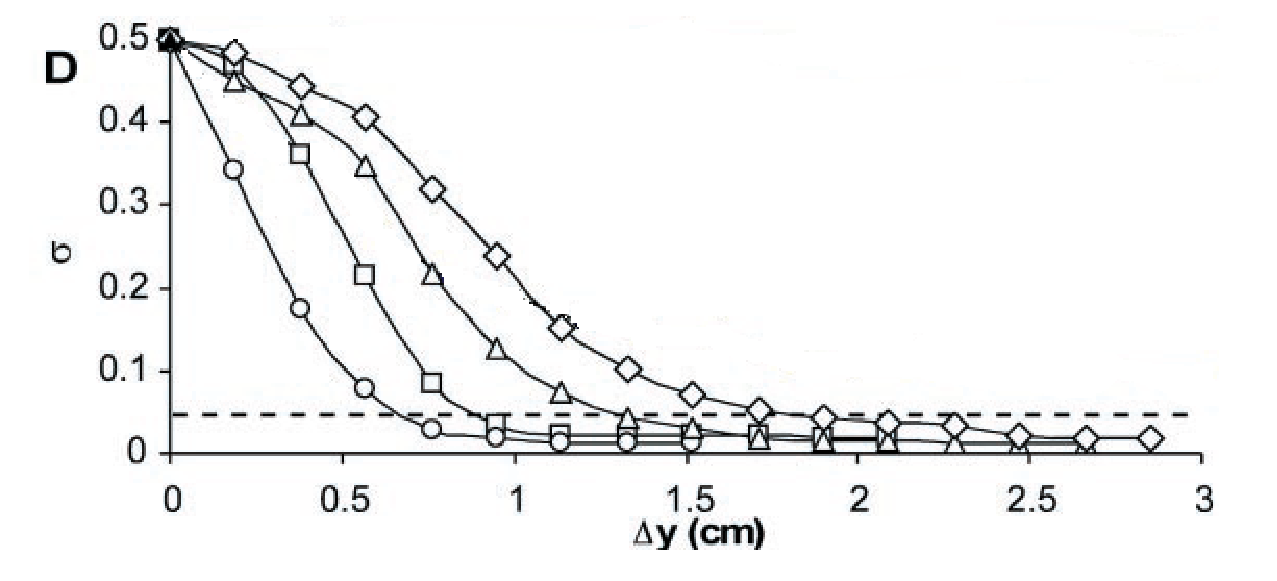
\includegraphics[width=1\textwidth]{stroockexperiment}
       \tiny{Stroock's Experiment. The largest $\text{Pe} = 9\times 10^5$.} 
       \end{center}
       \end{minipage}\hfill&
       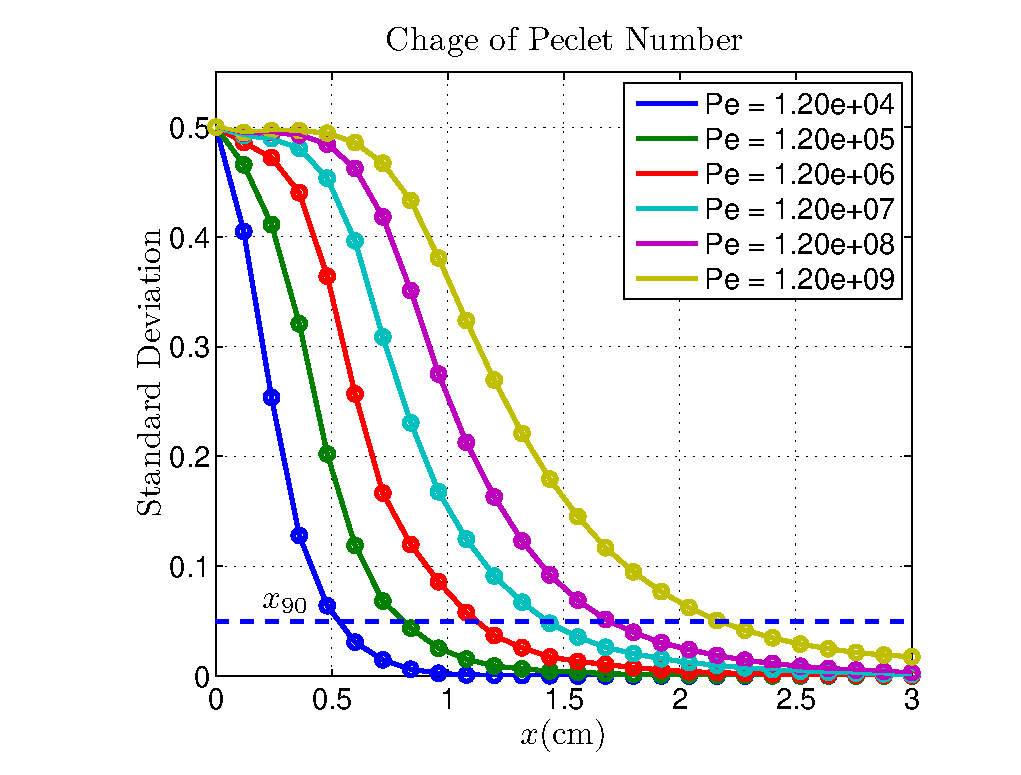
\includegraphics[width=0.47\textwidth]{example2veryPe2}      
    \end{tabular}
    \end{center}
 \begin{itemize}
       \item Half channel length $\neq$ half mixing.  
       \item Spectral Gap $1-|\lambda_2|$ does not always mean ``mixing rate''.       
 \end{itemize}
\end{frame}

%%%%%%%%%%%%%%%%%%%%%%%%%%%%%%%%%%%%%%%%%%%%%%%%%%%%%%%%%%
%%%%%%%%%%%%%%%%%%%%%%%%%%%%%%%%%%%%%%%%%%%%%%%%%%%%%%%%%%
\begin{frame}
 \myframetitle{Concluding Thoughts}
 \begin{itemize}
  
  \item Main achievements: 
    \begin{itemize}
    \item Showing how much benefit we can get from optimized microfluidic mixing channels.
    \item Providing numerical and analytical evidence for chaotic map cutoffs.
    \item Linking chaotic microfluidic mixing with the cutoff phenomenon.     
    \end{itemize}
  \item Open questions:
    \begin{itemize}
    \item Mixing in ocean and atmosphere.
    \item Chaotic search strategy effectiveness and cutoff.
    \item Can we detect cutoffs in simulation from a few trajectories?
    \end{itemize}
 \end{itemize}
\end{frame}


\end{document}
